\chapter{RankGen: Diagnostic Evaluation of Generative Models}
\label{ch:rankgen}

\section{Introduction and Motivation}
\label{sec:rankgen:intro}

Chapter~\ref{ch:theory} established the theoretical foundations for this
thesis, introducing graphs as structured data objects, reviewing
representation learning methods, and discussing the principles underlying
modern generative models. While these developments have enabled increasingly
powerful models for generating structured data, they also raise a fundamental
question: \emph{how should the quality of generative models be evaluated in a
way that is reliable, interpretable, and relevant to downstream tasks?}

Generative models are now widely used across domains such as image synthesis,
molecular design, graph generation, and natural language processing.
In many cases, these models produce samples that appear realistic or
domain-valid. However, visual or qualitative inspection alone is insufficient
for rigorous comparison between models, and reliable automated evaluation
remains an open challenge.

Many widely used evaluation metrics are brittle, easy to manipulate, and often
poorly aligned with the practical value of generated data. Standard metrics may
assign high scores to models that memorise training data, fail to generalise,
or provide little benefit in downstream predictive tasks. As a result, model
selection based solely on such scores can lead to unreliable conclusions and
potentially unsafe deployment decisions.

A large body of work has highlighted these limitations. Single-number
heuristics such as the Inception Score (IS)~\citep{salimans2016improved} and
Fr\'echet Inception Distance (FID)~\citep{heusel2017gans}, together with
kernel-based distances such as MMD and KID
\citep{gretton2012kernel,binkowski2018demystifying}, provide convenient scalar
summaries of generative performance. However, these metrics rely on strong
assumptions about feature representations and distributional structure.
In practice, they are sensitive to implementation choices, preprocessing
pipelines, and the particular feature extractor used to embed samples
\citep{barratt2018note,chong2020effectively,parmar2022aliased,
jayasumana2024rethinking,betzalel2022study}. Moreover, reducing generator
performance to a single scalar collapses distinct aspects of generative
behaviour---such as fidelity, diversity, and task relevance---and can obscure
important failure modes including mode collapse or data copying.

To address these limitations, several works propose multi-dimensional
evaluation summaries. Metrics such as precision--recall for distributions
\citep{sajjadi2018assessing,kynkaanniemi2019improved} and density--coverage
\citep{naeem2020reliable} attempt to separate aspects of fidelity and support,
providing more nuanced diagnostic information. Nevertheless, these approaches
remain strongly dependent on representation choices and typically lack
statistical guarantees about the reliability of the reported scores.Classifier-based evaluation protocols move closer to practical utility.
Methods such as GAN-train/test~\citep{shmelkov2018good} and
train-on-synthetic, test-on-real (TSTR)
\citep{hyland2017real,esteban2017real,yoon2019timegan} evaluate whether
generated data supports predictive tasks. However, these protocols are
typically reported as point estimates and provide little insight into the
statistical reliability of the observed results.

A particularly important risk is \textbf{memorisation}. Generative models may
replicate training data, artificially inflating similarity metrics while
providing little additional information and potentially exposing sensitive
training examples~\citep{bhattacharjee2023data}. Recent work has demonstrated
that diffusion and GAN models can leak training samples through extraction
attacks ~\citep{carlini2023extracting,hayes2019logan,chen2020ganleaks}, yet
many commonly used evaluation scores fail to detect such behaviour.

\begin{figure}[t]
  \centering
  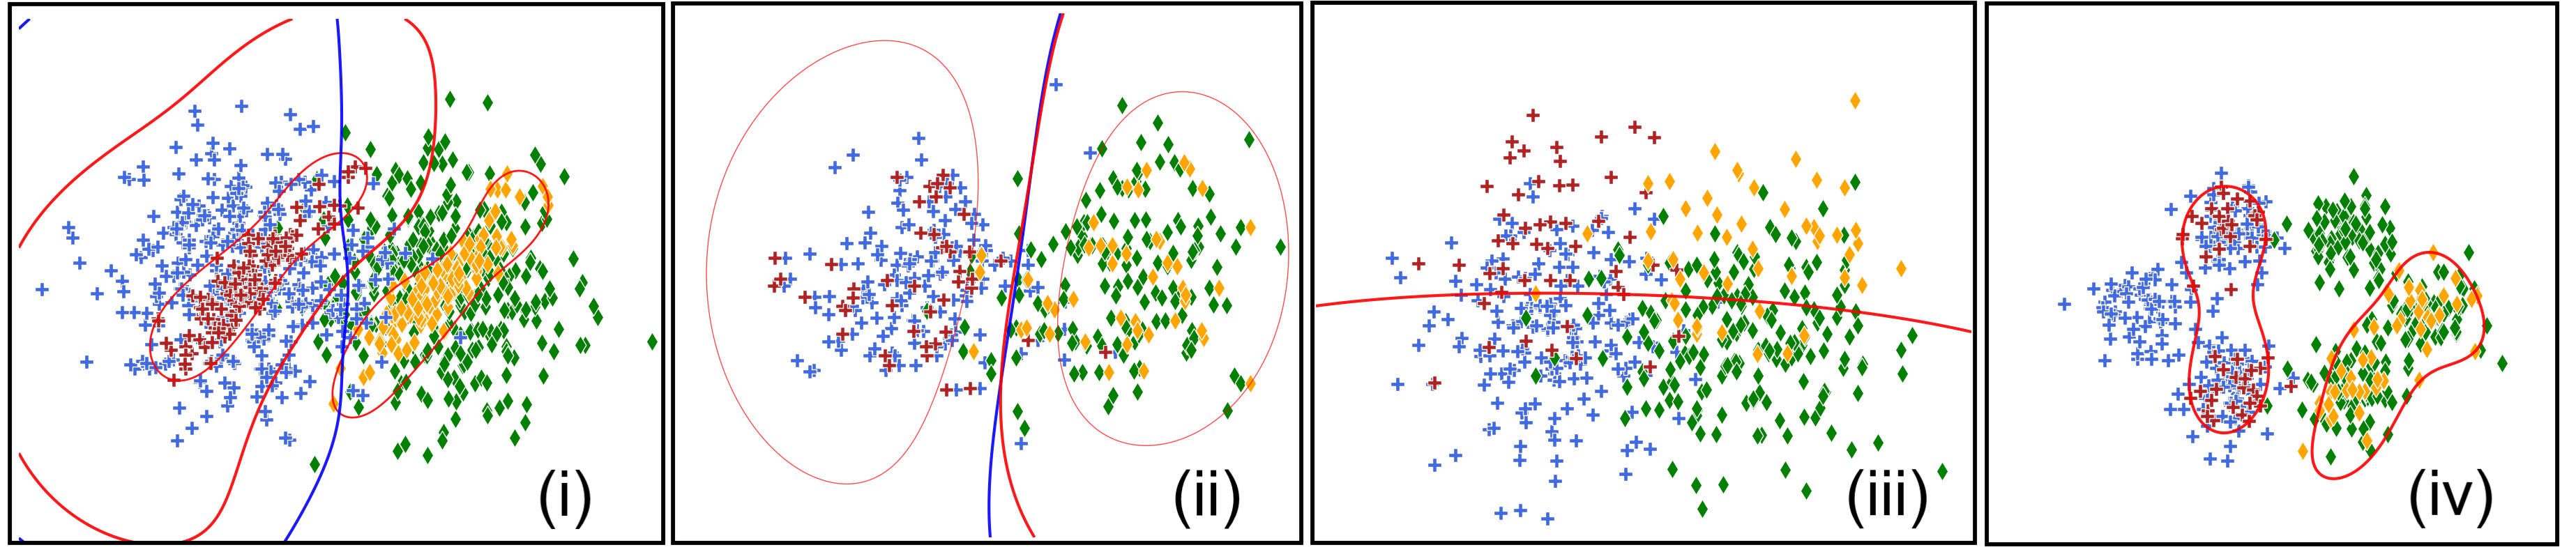
\includegraphics[width=1\linewidth]{images/rankgen/metrics.png}
  \caption{Four common generative failure modes and how RankGen detects them.
Each panel shows real data (blue and green) and generated data (red and orange)
for a binary classification task. Marker shapes denote classes.}
  \label{fig:generated-results}
\end{figure}
These challenges highlight a broader issue: generative model evaluation is
inherently multi-dimensional. A generator may preserve task-relevant signal,
yet still be easy to distinguish from real data. It may align globally with the
data distribution but fail to provide useful new information.

Figure
\ref{fig:generated-results} illustrates several such failure modes. Each panel shows real data (blue/green) and generated data (red/orange) for a binary classification task, with marker shapes indicating class labels. (i) \emph{Quality (poor task fidelity):} Generated samples lie in high-density regions of the real distribution but fail to produce a decision boundary that generalises, leading to poor classifier performance when trained on synthetic data. (ii) \emph{Utility (no added value):} Generated samples closely replicate the real data; augmenting the training set with them neither improves performance nor alters the decision boundary. (iii) \emph{Indistinguishability (easy to distinguish):} A subtle artefact (e.g., a shift in a single feature) allows a discriminator to separate real from generated samples, despite their apparent global similarity. (iv) \emph{Similarity (local mismatch):} Local neighbourhoods are dominated by either real or generated samples, indicating poor mixing due to structural differences or mode collapse; this is captured by neighbourhood entropy even when global distributions overlap.
\section{Limitations of Existing Evaluation Approaches}
\label{sec:rankgen:limitations}

Chapter~\ref{ch:theory} reviewed the principal families of metrics used to
evaluate generative models, including scalar heuristics, distributional
distances, and classifier-based evaluation protocols. While these approaches
provide useful insight, they also exhibit important limitations that make
reliable comparison between generative models difficult. In this section we
briefly revisit these approaches and highlight the specific shortcomings that
motivate the RankGen framework.

Many generative models are evaluated using single-number metrics such as the
Inception Score (IS)~\citep{salimans2016improved}, the Fr\'echet Inception
Distance (FID)~\citep{heusel2017gans}, or kernel-based distances such as
Maximum Mean Discrepancy (MMD) and Kernel Inception Distance (KID)
\citep{gretton2012kernel,binkowski2018demystifying}. These metrics are widely
used because they provide convenient scalar summaries that allow models to be
ranked easily.

However, such metrics rely on strong assumptions about the representation space
used to embed samples. Their values can vary substantially depending on the
choice of feature extractor, preprocessing pipeline, or evaluation protocol
\citep{barratt2018note,chong2020effectively,parmar2022aliased,betzalel2022study}.
Moreover, compressing generative behaviour into a single scalar inevitably
conflates multiple aspects of performance, including fidelity, diversity, and
task relevance. As a consequence, these metrics often fail to reveal important
failure modes such as mode collapse or data copying.

To address these shortcomings, several works propose multi-dimensional
evaluation summaries that separate different aspects of generative behaviour.
Examples include precision--recall for distributions
\citep{sajjadi2018assessing,kynkaanniemi2019improved} and density--coverage
metrics~\citep{naeem2020reliable}. These approaches provide richer diagnostic
information by distinguishing between fidelity and support coverage.

Despite these improvements, such metrics remain highly dependent on the
representation space used to compare samples. Small changes in embedding
choices or feature extraction pipelines can significantly alter the reported
scores. Furthermore, most of these methods remain descriptive rather than
inferential: they quantify differences between datasets but rarely provide
statistical guarantees regarding the reliability of the observed comparisons.

A different line of work evaluates generative models through predictive tasks.
Protocols such as GAN-train/test~\citep{shmelkov2018good} and
train-on-synthetic, test-on-real (TSTR)
\citep{hyland2017real,esteban2017real,yoon2019timegan} measure whether
generated data supports supervised learning tasks. This perspective is
particularly appealing because it directly relates generative performance to
downstream predictive utility.

However, these evaluations are typically reported as point estimates without
uncertainty quantification. Differences between models may therefore reflect
sampling noise or training variability rather than genuine differences in
generative quality. In addition, a single predictive score often conflates
multiple potential failure modes, such as insufficient diversity, poor signal
fidelity, or overfitting to the training data.

An especially problematic failure mode is memorisation. Generative models may
reproduce training samples or near-duplicates, artificially inflating
similarity metrics while contributing little additional information.
Beyond limiting the usefulness of generated data, memorisation also raises
important privacy concerns when sensitive training samples can be reconstructed
or extracted from a trained generator
\citep{bhattacharjee2023data,carlini2023extracting,hayes2019logan,chen2020ganleaks}.
Many widely used evaluation protocols fail to detect such behaviour.

Taken together, these observations reveal that existing evaluation approaches
provide only partial insight into the behaviour of generative models.
Scalar metrics are simple but brittle, distributional diagnostics are more
informative but representation-dependent, and classifier-based evaluations
align with practical utility but lack statistical guarantees.

These limitations motivate the RankGen framework developed in this chapter:
an evaluation protocol that uses predictive probes to separate different
failure modes, attaches reliability checks to the resulting estimates, and
uses robust summaries when comparing generators.

\section{RankGen Contribution and Chapter Structure}
To address these challenges, this chapter introduces \textbf{RankGen}, a
classifier-based evaluation framework that treats generator assessment as a
set of predictive probes. The framework defines four metrics: \emph{Quality}
(signal fidelity), \emph{Utility} (added predictive value beyond real data),
\emph{Indistinguishability} (two-sample alignment), and \emph{Similarity}
(local structural mixing between real and generated samples). Each metric is
paired with a PAC-style reliability check for the corresponding empirical
estimate. Candidate generators are then evaluated through a four-stage
protocol: data preparation, probe training, reliability filtering, and robust
ranking. A composite score, \emph{Exchangeability}, aggregates the accepted
signals to summarise predictive usefulness and distributional alignment.

The contribution of the chapter is therefore not another single score, but a
diagnostic protocol for asking which aspect of generation fails, whether the
evidence is reliable under the chosen probes, and how surviving models should
be ranked across repeated evaluations. The empirical sections test this
protocol on controlled perturbations, molecular graph generators, image
benchmarks, and open-domain text generation.

\paragraph{Chapter structure.}
The remainder of this chapter is organised as follows. The preceding section
identified limitations of existing evaluation approaches and motivated the need
for a diagnostic framework with explicit reliability checks.
Section~\ref{sec:rankgen:framework} reformulates generative model evaluation
as a learning problem.
Section~\ref{sec:method} presents the RankGen methodology, including the data
preparation pipeline, classifier-based probes, PAC-style guarantees,
quantile-based aggregation, and the ranking procedure.
Section~\ref{sec:empirical} reports empirical results on controlled synthetic
perturbations, molecular graph datasets, image benchmarks, and open-domain
text generation.
Finally, Section~\ref{sec:conclusion-rankgen} concludes the chapter and
summarizes its main findings.



\section{Evaluation as a Learning Problem}
\label{sec:rankgen:framework}

The limitations of existing evaluation metrics suggest that assessing
generative models cannot be reduced to computing a single similarity score
between real and generated datasets. Instead, evaluation must capture how
generated samples interact with real data in tasks that reflect the intended
use of the generator.

A useful perspective is to view generative model evaluation through the lens
of statistical learning theory. In this view, generated samples are treated as
data produced by an alternative distribution, and evaluation is formulated as
a collection of predictive tasks designed to probe different aspects of the
relationship between the generated and real distributions.

Let $P_r$ denote the real data distribution and $P_g$ the distribution induced
by a generative model.
by a generative model. Given samples from these distributions, we construct
learning problems whose solutions reveal properties of the generator.
Different predictive tasks expose different types of failure modes.

For example, if a classifier trained on generated data generalises poorly to
real data, this suggests that the generator fails to capture task-relevant
structure. Conversely, if a classifier can easily distinguish real from
generated samples, this indicates a distributional mismatch between $D_r$ and
$D_g$. If generated samples provide no improvement when added to real training
data, this suggests that the generator contributes little new information.

This perspective leads naturally to the idea of \emph{evaluation probes}.
Each probe is a supervised learning problem designed to measure a specific
property of the generator. By observing how predictive models behave under
different training configurations involving real and generated data, it is
possible to infer properties of the underlying generative distribution.

Importantly, framing evaluation in this way enables the use of tools from
learning theory to reason about reliability. Instead of reporting raw
empirical scores, evaluation results can be accompanied by statistical
generalisation guarantees that bound the discrepancy between observed
performance and true performance on unseen data.

Within this framework, generative model evaluation becomes a structured
procedure consisting of multiple predictive probes, each targeting a
different potential failure mode.

\section{The Method: RankGen}
\label{sec:method}

\textbf{RankGen} evaluates generative models through a statistically grounded,
classifier-based framework that jointly measures predictive usefulness and
distributional alignment. Rather than relying on a single similarity score,
RankGen decomposes evaluation into complementary probes and combines them
with PAC-style guarantees and robust statistical summaries.

Evaluating generative models requires balancing \emph{reliability} and
\emph{resolution}. RankGen explicitly separates these roles:
(i) \emph{PAC-style bounds} act as \emph{reliability gates}, ensuring that
reported scores hold with high probability, and
(ii) \emph{quantile-based summaries} (median and IQR) provide resolution,
capturing central tendency and variability across stochastic trials.
Together, these prevent unreliable models from being ranked while enabling
fine-grained comparison among valid ones.

\paragraph{Pipeline overview.}
RankGen follows a four-stage evaluation pipeline:

\textbf{(1) Data preparation and sampling.}
We generate multiple stochastic replicates using stratified bootstrap splits of
the labelled dataset. For each replicate, we construct
$D_{\text{train1}}^{(i)}$, $D_{\text{train2}}^{(i)}$, and a fixed
$D_{\text{test}}$. Generators are trained on
$D_{\text{train1}}^{(i)}$ and produce class-conditional synthetic samples,
yielding $D_{\text{generated}}^{(i)}$.

\textbf{(2) Metric evaluation.}
We evaluate generators using four classifier-based probes:
\emph{Quality} (signal fidelity),
\emph{Utility} (added predictive value),
\emph{Indistinguishability} (real vs.\ generated separability), and
\emph{Similarity} (local structural mixing).
Each metric captures a distinct failure mode and is computed under a unified
evaluation protocol.

\textbf{(3) Statistical aggregation.}
For each metric, we compute PAC-style generalisation bounds to ensure
statistical reliability, and aggregate results across replicates using robust
quantile summaries (median and IQR). This yields stable, uncertainty-aware
estimates of generator performance.

\textbf{(4) Ranking and diagnosis.}
We first filter generators based on bound violations (pass/fail per metric),
retaining only statistically reliable candidates. Within each group, models
are ranked using quantile summaries and pairwise dominance. Finally, the joint
metric profile is used for \emph{diagnosis}: for example, high similarity but
low utility indicates copying, while high quality but low indistinguishability
suggests distributional mismatch.

\medskip
This multi-dimensional view enables RankGen to move beyond scalar evaluation,
providing both reliable ranking and interpretable insights into how and why
generators succeed or fail.
\begin{figure}[H]
    % \centering
    \hspace{-1.25cm}
    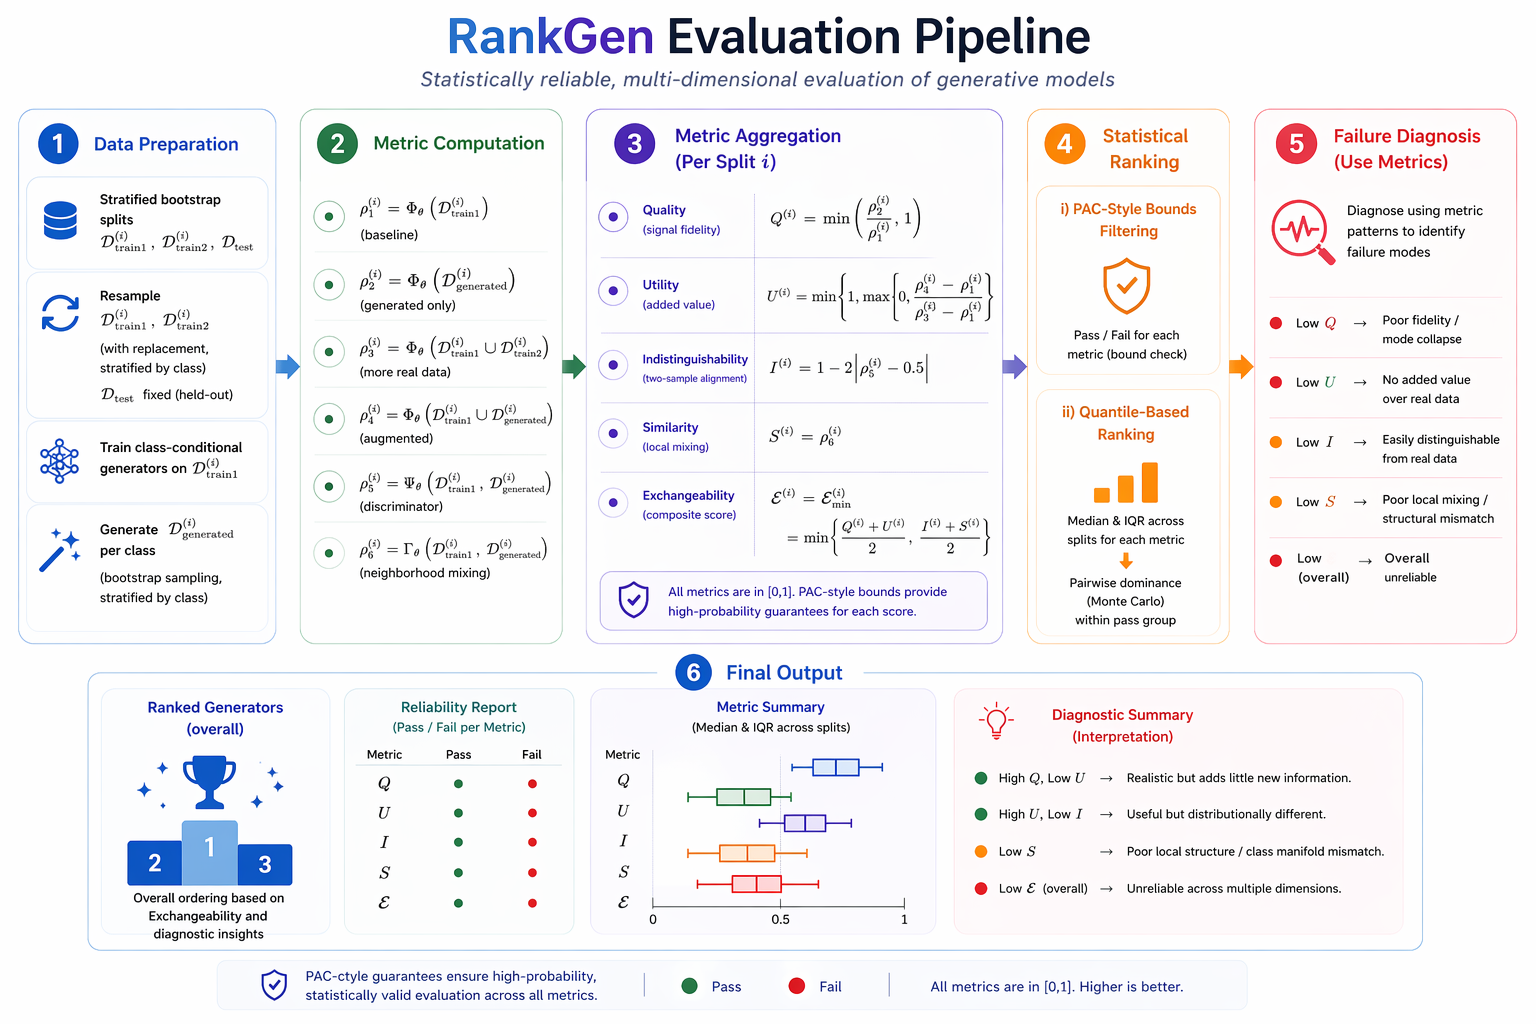
\includegraphics[width=1.25\linewidth]{images/rankgen/pipeline_final.png}
    \caption{
    \textbf{RankGen evaluation pipeline.}
    The framework consists of four stages:
    (1) \emph{Data preparation} via stratified bootstrap splits and class-conditional generation;
    (2) \emph{Metric evaluation} using classifier-based probes (Quality, Utility, Indistinguishability, Similarity);
    (3) \emph{Statistical aggregation} combining PAC-style reliability bounds with quantile summaries;
    and (4) \emph{Ranking and diagnosis}, where generators are filtered by pass/fail checks and ranked using robust statistics, with metric profiles used to diagnose failure modes.
    }
    \label{fig:rankgen_pipeline}
\end{figure}
%-------------------------------------------------------------------------------------------------------------
\subsection{Data Preparation and Sampling}

Consider a classification dataset \(D = \{(x_i, y_i)\}_{i=1}^N\),
where each feature vector \(x_i \in \mathbb{R}^d\) lies in a \(d\)-dimensional space,
and each label \(y_i \in \{1,\ldots,C\}\) denotes one of \(C\) classes.
We first partition \(D\) into a training set \(D_{\text{train}}\) and a held-out
test set \(D_{\text{test}}\).
The training set is then further divided, using stratified sampling, into two
equally sized subsets, \(D_{\text{train1}}\) and \(D_{\text{train2}}\).


\paragraph{Training the generators.}
We adopt a class-wise strategy for generating synthetic data.
Unless the underlying model is inherently class-conditional, we train a separate
generator for each class.
Specifically, for every class \(c \in \{1,\ldots,C\}\), we fit a generative model \(f_c\) using only
the corresponding subset \(D_{\text{train1}}^{c}\) of the training data.
For models that are unconditional, we use the same generator architecture,
but train it independently on the samples of each class.
%Each generator is trained once per generator configuration, and is not retrained across replicates.


\paragraph{Constructing the synthetic pool.}
After training, we draw synthetic samples once for each class to construct a
base synthetic dataset. Let \(p_{f_c}\) denote the distribution induced by the generator \(f_c\). For each class \(c\), we sample
$
\{x_{c,\ell}\}_{\ell=1}^{N_c} \sim p_{f_c},
$ where \(N_c = |D_{\text{train1}}^{c}|\) is the desired number of generated examples for class \(c\).
The resulting synthetic dataset is then the union of all class specific samples
\[
D_{\text{generated}}
= \bigcup_{c}
\{(x_{c,\ell},\, c) : \ell = 1,\ldots,N_c\}.
\]



\paragraph{Uncertainty estimate.}
To estimate uncertainty for each replicate \(i\), we draw bootstrap samples
$
D_{\text{train1}}^{(i)} \subseteq D_{\text{train1}},\quad
D_{\text{train2}}^{(i)} \subseteq D_{\text{train2}},\quad
D_{\text{generated}}^{(i)} \subseteq D_{\text{generated}},\quad
$
using class-stratified bootstrapping.
Each replicate is used to compute all four metrics and their quantile summaries.


%-------------------------------------------------------------------------------------------------------------
\subsection{Classifier Performance Scores (\texorpdfstring{$\rho_i$}{rho\_i})}
We propose 4 key metrics: Quality, Utility, Indistinguishability, and Similarity defined via classifier-derived scores $\rho^{(i)}_j$ (Table~\ref{tab:classifier-metrics}), with every score corresponding to a distinct training-and-testing configuration on split $i$. All models are evaluated on the same shared test set $D_{\text{test}}$. Here, $\Phi_\theta$ denotes a task classifier, $\Psi_\theta$ a binary real-vs-generated discriminator, and $\Gamma_\theta$ a structure-aware similarity model (e.g., a data-specific kernel).

\begin{table}[H]
\centering
\caption{Classifier-based evaluation metrics used in \textsc{RankGen}.}
\label{tab:classifier-metrics}
\begin{small}
\begin{tabular}{@{}l p{0.65\linewidth}@{}}  % <-- wrap description
\toprule
\textbf{Metric} & \textbf{Description} \\
\midrule
$\rho_1^{(i)} = \Phi_{\theta}(D_{\text{train1}}^{(i)})$ & Accuracy of classifier trained on real data only (baseline). \\
$\rho_2^{(i)} = \Phi_{\theta}(D_{\text{generated}}^{(i)})$ & Accuracy when trained on generated data only (signal fidelity). \\
$\rho_3^{(i)} = \Phi_{\theta}(D_{\text{train1}}^{(i)} \cup D_{\text{train2}}^{(i)})$ & Accuracy with extra real data (upper bound). \\
$\rho_4^{(i)} = \Phi_{\theta}(D_{\text{train1}}^{(i)} \cup D_{\text{generated}}^{(i)})$ & Accuracy with real+generated data (usefulness). \\
$\rho_5^{(i)} = \Psi_{\theta}(D_{\text{train1}}^{(i)}, D_{\text{generated}}^{(i)})$ & Discriminator accuracy distinguishing real vs.\ generated. \\
$\rho_6^{(i)} = \Gamma_{\theta}(D_{\text{train1}}^{(i)}, D_{\text{generated}}^{(i)})$ & Entropy-based similarity of local feature neighbourhoods. \\
\bottomrule
\end{tabular}
\end{small}
\end{table}



%---------------------------------------------------------------------------------------------------------
\subsection{Quality Metric}
\label{sec:quality}

\paragraph{Definition (normalized TSTR).}
The \textbf{quality} score quantifies how much predictive signal synthetic data
carries relative to real data. On split $i$, let $\rho^{(i)}_1$ be the task
score (e.g., accuracy, AUC, or macro-F1) of a classifier $\Phi_\theta$ trained
on $D^{(i)}_{\text{train1}}$ and evaluated on $D_{\text{test}}$, and let
$\rho^{(i)}_2$ be the score of the same classifier class trained on
$D^{(i)}_{\text{generated}}$ and evaluated on $D_{\text{test}}$. We define the
normalized Train-on-Generated-Test-on-Real (TSTR) ratio
\[
Q^{(i)} := \min\!\left(\frac{\rho^{(i)}_2}{\rho^{(i)}_1},\,1\right)\in[0,1].
\]

\paragraph{generalisation bound.}
Using the PAC-learning preliminaries introduced in Chapter~\ref{ch:theory},
together with a standard domain-adaptation argument, one obtains a conservative
lower bound on the population quality score in terms of three quantities:
(i) generalisation error for the task classifier, (ii) discrepancy between the
real and generated distributions, and (iii) the joint optimal risk between the
two domains. The resulting guarantee shows that quality degrades as classifier
uncertainty or distributional mismatch increases. A full derivation and exact
bound statement are given in Appendix~\ref{app:theory-quality}.

\paragraph{Interpretation and practice.}
High values close to $1$ indicate that synthetic data preserves task-relevant
structure, whereas low values reveal fidelity gaps such as label noise, mode
collapse, or covariate shift. Any bounded task score in $[0,1]$ may be used,
but the \emph{same} score must define both $\rho^{(i)}_1$ and $\rho^{(i)}_2$ to
ensure comparability; for imbalanced labels, macro-averaged variants are often
preferable. When the real-data baseline $\rho^{(i)}_1$ is close to chance, the
ratio becomes unstable and the bound loosens; in practice, we either enforce a
minimal baseline before reporting the ratio or report the ratio alongside the
absolute scores. Across resampling trials, we aggregate $Q^{(i)}$ using robust
quantiles (median and IQR; see Sec.~\ref{sec:quantile-based-estimation}) and
use the PAC bound as a pass/fail gate prior to fine-grained ranking. If
training on synthetic data outperforms training on real
($\rho^{(i)}_2>\rho^{(i)}_1$), we cap the score at $1$ for consistency with the
other $[0,1]$ metrics used in the composite, while retaining the uncapped ratio
for diagnostic analysis if needed.


%---------------------------------------------------------------------------------------------------------
\subsection{Utility Metric}
\label{sec:utility}

\paragraph{Definition.}
The \emph{utility} score quantifies the incremental benefit of augmenting real
training data with synthetic samples. Let
\[
\Delta_{\mathrm{real}}^{(i)} := \rho_3^{(i)}-\rho_1^{(i)}
\]
denote the gain from adding more \emph{real} data, and let
\[
\Delta_{\mathrm{generated}}^{(i)} := \rho_4^{(i)}-\rho_1^{(i)}
\]
denote the gain from adding \emph{generated} data under the same augmentation
budget. We define
\[
U^{(i)} \;=\;
\min\!\Bigl\{1,\;\max\!\bigl\{0,\;
\Delta_{\mathrm{generated}}^{(i)} / \Delta_{\mathrm{real}}^{(i)}
\bigr\}\Bigr\},
\]
so that values near $1$ indicate that synthetic data is nearly as useful as
additional real data. For diagnostic purposes, we also retain the uncapped ratio
\[
\tilde U^{(i)}=
\Delta_{\mathrm{generated}}^{(i)} / \Delta_{\mathrm{real}}^{(i)}.
\]

\paragraph{Generalisation bound.}
Using the PAC-learning preliminaries from Chapter~\ref{ch:theory}, together
with a standard domain-adaptation argument, one obtains a conservative lower
bound on the population utility score in terms of three quantities: (i)
generalisation error of the task classifiers, (ii) discrepancy between the real
and generated distributions, and (iii) the joint optimal risk across the two
domains. Intuitively, the guarantee becomes weaker when generated samples are
easy to distinguish from real ones or when the gain from extra real data is very
small. A full derivation and exact bound statement are given in
Appendix~\ref{app:theory-utility}.

\paragraph{Interpretation and practice.}
Utility captures whether synthetic data contributes \emph{additional} predictive
value beyond the original real training set. When a generator merely memorises
existing samples, synthetic augmentation adds little or no new information, so
$\Delta_{\mathrm{generated}}^{(i)}$ remains small and $U^{(i)}$ collapses
toward $0$, even if other similarity-style scores appear strong. Conversely,
when the synthetic distribution is both well aligned with the real one and rich
in task-relevant variation, the gain from augmentation approaches that obtained
from additional real data, pushing $U^{(i)}$ toward $1$.

In reporting, we keep augmentation budgets matched between real and synthetic
additions, use the \emph{same} bounded task score for all $\rho_j^{(i)}$
involved, and aggregate $U^{(i)}$ across resamples using robust quantiles
(median and IQR; see Sec.~\ref{sec:quantile-based-estimation}). As with the
other metrics, we use the PAC bound as a pass/fail gate prior to fine-grained
ranking. Two practical cautions are important. First, if
$\Delta_{\mathrm{real}}^{(i)}$ is very small, the ratio becomes unstable; in
that case, we report the absolute gains alongside the ratio or revert to the
difference form discussed in Appendix~\ref{app:theory-utility}. Second, if
synthetic augmentation helps more than additional real data
($\tilde U^{(i)}>1$), we cap the reported score at $1$ for comparability in the
composite metric while retaining $\tilde U^{(i)}$ for diagnosis.
%---------------------------------------------------------------------------------------------------------
%---------------------------------------------------------------------------------------------------------
\subsection{Indistinguishability Metric}
\label{sec:indistinguishability}

\paragraph{Definition.}
Indistinguishability measures how difficult it is for a discriminator
$\Psi_\theta$ to distinguish real samples from generated ones on a held-out,
balanced evaluation set. Let $\rho^{(i)}_5$ denote the test accuracy of the
real-vs-generated discriminator on split $i$, where chance performance is
$0.5$. We define the symmetric score
\[
I^{(i)} \;=\; 1 - 2\bigl|\rho^{(i)}_5 - 0.5\bigr| \;\in\; [0,1],
\]
so that $I^{(i)}=1$ when the discriminator operates at chance, indicating that
real and generated samples are hard to separate, and $I^{(i)}=0$ when the two
domains are perfectly distinguishable. For diagnostic purposes, one may also
report the conventional quantity $1-\rho^{(i)}_5$, but we use the symmetric
mapping above to keep all base metrics on a common $[0,1]$ scale. The same
definition can also be applied with AUC in place of accuracy.

\paragraph{Generalisation bound.}
Using the PAC-learning preliminaries from Chapter~\ref{ch:theory}, standard
uniform-convergence arguments for the discriminator imply that, with
probability at least $1-\delta$, the empirical discriminator accuracy remains
close to its population counterpart. Since the mapping
$x \mapsto 1-2|x-0.5|$ is Lipschitz on $[0,1]$, the same control transfers
directly to the indistinguishability score. A full statement and derivation are
given in Appendix~\ref{app:theory-indistinguishability}.

\paragraph{Interpretation and practice.}
High values of $I^{(i)}$ indicate that generated samples are difficult to
distinguish from real ones, suggesting strong global alignment between the two
distributions. Low values indicate that the generator leaves detectable
artefacts or systematic shifts that a discriminator can exploit. This metric is
therefore complementary to the predictive probes: a generator may support good
task performance while still being distributionally distinguishable, or vice
versa.

Two practical considerations are especially important. First, discriminator
capacity must be controlled carefully. An overly expressive discriminator may
pick up trivial cues, such as preprocessing artefacts or metadata leakage,
rather than meaningful distributional differences. Second, evaluation should be
balanced and use identical preprocessing for real and generated data. When
class imbalance makes accuracy less appropriate, AUC is preferable, together
with the same symmetric transformation above. Across resampling trials, we
aggregate $I^{(i)}$ using robust quantiles (median and IQR; see
Sec.~\ref{sec:quantile-based-estimation}) and use the corresponding PAC bound
as a reliability gate prior to fine-grained ranking.


%---------------------------------------------------------------------------------------------------------
%---------------------------------------------------------------------------------------------------------
\subsection{Similarity Metric}
\label{sec:similarity}

\paragraph{Definition.}
Similarity measures \emph{local mixing} between real and generated samples.
Let $D_{\mathrm{mix}}^{(i)}=D_{\mathrm{train1}}^{(i)} \cup D_{\mathrm{generated}}^{(i)}$
with $n=|D_{\mathrm{mix}}^{(i)}|$.
For each $x\in D_{\mathrm{mix}}^{(i)}$, let $\mathcal N_k(x)$ be its $k$
nearest neighbours (excluding $x$ and breaking ties deterministically),
computed in the same feature space used by the task classifier.
Define the local domain proportion
\[
\hat p_x \;=\; \frac{1}{k}\sum_{z\in \mathcal N_k(x)}
\mathbf{1}\{\mathrm{dom}(z)=\mathrm{dom}(x)\},
\]
and map it to a unit-interval score using the binary entropy
$H(p)=-p\log p-(1-p)\log(1-p)$. The empirical similarity on split $i$ is
\[
S^{(i)} \;=\;
\frac{1}{n}\sum_{x\in D_{\mathrm{mix}}^{(i)}}
\frac{H(\hat p_x)}{\log 2}
\;\in\; [0,1],
\]
with population counterpart
$S^\star=\mathbb E_{x\sim D_{\mathrm{mix}}}[H(p_x)/\log 2]$.
\footnote{A linear alternative, $1-2\lvert \hat p_x-\tfrac12\rvert$, is also
admissible; the entropy mapping stabilizes estimates near
$\hat p_x\!\approx\!0.5$ and downweights extreme but noisy values.}

\paragraph{Generalisation bound.}
Neighbourhood label proportions are computed from samples drawn without
replacement, so their deviations are governed by hypergeometric
concentration inequalities. Combined with the Lipschitz continuity of the
entropy mapping and a union bound over all points, this yields a
high-probability bound controlling the deviation of $S^{(i)}$ from its
population value. The resulting error decreases with increasing neighbourhood
size $k$ and sample size $n$, and depends explicitly on $\log k$ through the
Lipschitz constant. A full derivation and exact bound are given in
Appendix~\ref{app:theory-similarity}.

\paragraph{Interpretation and practice.}
High similarity (values near $1$) indicates that real and synthetic samples
interleave in local neighbourhoods, as expected when the generator captures
the geometry of the real distribution without introducing systematic shifts.
Low values indicate domain-segregated regions and typically reflect mode
collapse or geometric misalignment.

In practice, the choice of $k$ trades bias for variance: larger $k$ stabilizes
the local proportion estimates but may blur fine-scale structure, while small
$k$ captures local geometry at the cost of higher variance. We typically select
$k$ in the range $[10,50]$ and report sensitivity where appropriate. To reduce
small-sample noise, a leave-one-out convention and mild shrinkage
(e.g., $\tilde p_x=\frac{c+\sum \mathbf{1}\{\cdot\}}{2c+k}$ with
$c=\tfrac12$) can be effective.

Because locality depends on the feature space, distances should be computed in
a task-relevant embedding (e.g., the same features used to train
$\Phi_\theta$), with identical preprocessing applied to real and generated
data to avoid artefactual cues. Similarity complements indistinguishability:
a generator may be globally hard to distinguish yet locally segregated, or
locally well mixed yet provide little new information. The latter case is
captured by low utility (Sec.~\ref{sec:utility}), ensuring that copying or
near-duplication is not rewarded in the overall evaluation.

%---------------------------------------------------------------------------------------------------------
\subsection{Exchangeability Metric}
\label{sec:exchangeability}

\paragraph{Motivation.}
Practitioners often seek a single headline score to compare generators, yet
our four probes—\emph{Quality} $(Q^{(i)})$ and \emph{Utility} $(U^{(i)})$ for predictive value, and
\emph{Indistinguishability} $(I^{(i)})$ and \emph{Similarity} $(S^{(i)})$ for distributional alignment—capture
complementary aspects. A suitable composite should reward balanced performance
and be limited by the weakest dimension, reflecting that a generator is only as
useful as its least satisfactory property.

\paragraph{Definition.}
After mapping each base metric to $[0,1]$, define the predictive and
distributional blocks
\[
\Delta_{\mathrm{qual}}^{(i)} = \tfrac12\bigl(Q^{(i)}+U^{(i)}\bigr),
\qquad
\Delta_{\mathrm{sim}}^{(i)} = \tfrac12\bigl(I^{(i)}+S^{(i)}\bigr).
\]
We define the exchangeability score as
\[
\mathcal{E}^{(i)} \;\equiv\;
\mathcal{E}_{\min}^{(i)} \;=\;
\min\!\left\{\Delta_{\mathrm{qual}}^{(i)},\,
\Delta_{\mathrm{sim}}^{(i)}\right\}
\;\in\; [0,1].
\]
This definition ensures that strong performance along one axis cannot compensate
for weakness along the other: the score is driven by the limiting factor.

\paragraph{PAC guarantee.}
Suppose the PAC analyses of the four base metrics yield, with probability at
least $1-\delta$, bounds of the form
\[
Q^{(i)} \ge 1-\varepsilon_Q,\quad
U^{(i)} \ge 1-\varepsilon_U,\quad
I^{(i)} \ge 1-\varepsilon_I,\quad
S^{(i)} \ge 1-\varepsilon_S.
\]
Then, by linearity of the block averages and monotonicity of the minimum,
\[
\mathcal{E}_{\min}^{(i)}
\;\ge\;
1-\max\!\left\{
\tfrac{\varepsilon_Q+\varepsilon_U}{2},\;
\tfrac{\varepsilon_I+\varepsilon_S}{2}
\right\}.
\]
This provides a conservative PAC-style guarantee for the composite score; the
full derivation is given in Appendix~\ref{app:theory-exchangeability}.

\paragraph{Interpretation and practice.}
$\mathcal{E}_{\min}^{(i)}$ acts as a \emph{fail-safe} summary: a generator that
is locally well mixed but contributes no new information (copying) will exhibit
high similarity but low utility, lowering the predictive block and thus the
composite. Conversely, a generator that improves predictive performance while
remaining easily distinguishable will be penalized through the distributional
block.

In practice, we first apply the PAC-based reliability gates for each base
metric, then aggregate $\mathcal{E}_{\min}^{(i)}$ across resampled splits using
robust quantiles (median and IQR; see
Sec.~\ref{sec:quantile-based-estimation}). The composite serves as the primary
ranking score, while the individual components $(Q,U,I,S)$ diagnose which axis
limits performance.

\paragraph{Variants.}
When asymmetric weighting is desired, one may define
\[
\min\!\bigl\{\alpha\,\Delta_{\mathrm{qual}}^{(i)},\,
(1-\alpha)\,\Delta_{\mathrm{sim}}^{(i)}\bigr\},
\quad \alpha\in(0,1).
\]
For differentiable optimisation, a soft minimum
\[
\operatorname{smin}_\tau(a,b)
= -\tau \log\bigl(e^{-a/\tau}+e^{-b/\tau}\bigr),
\quad \tau>0,
\]
can approximate $\min(a,b)$ while improving numerical stability. We use the
hard minimum to preserve the conservative, safety-first semantics of the
composite.

%-------------------------------------------------------------------------------------------------------------
%-------------------------------------------------------------------------------------------------------------
\subsection{Quantile-Based Estimation}
\label{sec:quantile-based-estimation}

Performance across resampled splits can be heavy-tailed or even multimodal,
making mean$\pm$standard deviation summaries brittle. We therefore adopt
\emph{quantile-based} summaries for each metric and generator. Given the
empirical distribution of scores $\{Z^{(i)}\}_{i=1}^{B} \quad \text{(for a given metric } Z \in \{Q,U,I,S,\mathcal{E}_{\min}\})$ across resamples, we
compute the first quartile $Q_1$, median $M$, and third quartile $Q_3$, and
report the median together with the interquartile range
$\mathrm{IQR}=Q_3-Q_1$ as robust measures of location and dispersion.

For compatibility with methods that require moment-based summaries, we also
compute a \emph{pseudo-mean} and \emph{pseudo-standard deviation} using the
quantile-to-moment conversions of \citet{wan2016estimatingsamplemeanstandard}:
\[
\hat{\mu}_Q=\tfrac{Q_1+M+Q_3}{3},
\qquad
\hat{\sigma}_Q=\frac{\mathrm{IQR}}{1.34898},
\]
where $1.34898 = 2\,\Phi^{-1}(0.75)$ is the normal-reference constant linking
IQR and standard deviation. These estimates remain stable under skew and are
robust to outliers; however, we treat the median and IQR as the primary
descriptors, using $(\hat{\mu}_Q,\hat{\sigma}_Q)$ only as auxiliary summaries.

Because all base metrics are bounded in $[0,1]$, we clip trial scores to this
range prior to summarization. When uncertainty-aware ranking requires
sampling-based approximations, we draw from a truncated Gaussian
$\mathcal{N}(\hat{\mu}_Q,\hat{\sigma}_Q^2)$ restricted to $[0,1]$. To avoid
degenerate dispersion, we apply a small ridge
$\hat{\sigma}_Q \leftarrow \max\{\hat{\sigma}_Q,\tau\}$ with $\tau>0$
(we use $\tau=10^{-4}$ in experiments).

These robust summaries are used throughout for aggregation and ranking
(Secs.~\ref{sec:exchangeability} and~\ref{sec:ranking-across-metrics}).
A consolidated notation table and full derivations of the PAC-style bounds
are provided in Appendix~\ref{app:theory}; see in particular
Table~\ref{tab:notation-glossary} and
Appendices~\ref{app:theory-quality}--\ref{app:theory-exchangeability}.
%-------------------------------------------------------------------------------------------------------------
\subsection{Ranking Procedure}
\label{sec:ranking-across-metrics}

\textsc{RankGen} adopts a two-stage ranking procedure that balances statistical reliability with resolution. In the first stage, we apply PAC-style bounds to each generator--metric pair to determine whether the empirical score exceeds a theoretical threshold with high confidence. This yields a binary pass/fail outcome for each metric (as shown in Table~\ref{tab:bounds_check}), allowing us to group generators by the number of metrics they satisfy. Generators that fail fewer bounds are considered more trustworthy and are placed in higher-priority groups.
\begin{table}[H]
\centering
\scriptsize
\renewcommand{\arraystretch}{1.15}
\setlength{\tabcolsep}{5pt}

\rowcolors{2}{white}{gray!5}
\begin{tabular}{lccccc}
\toprule
\textbf{Generator}
& \textbf{Quality}
& \textbf{Utility}
& \shortstack{\textbf{Indistinguish} \\ \textbf{ability}}
& \textbf{Similarity}
& \shortstack{\textbf{Exchange-} \\ \textbf{ability}} \\
\midrule
s4dd\_u\_1  & \cellcolor{passblue}\cmark & \cellcolor{passblue}\cmark & \cellcolor{passblue}\cmark & \cellcolor{passblue}\cmark & \cellcolor{passblue}\cmark \\
s4dd\_u\_m  & \cellcolor{passblue}\cmark & \cellcolor{passblue}\cmark & \cellcolor{passblue}\cmark & \cellcolor{passblue}\cmark & \cellcolor{passblue}\cmark \\
stgg        & \cellcolor{passblue}\cmark & \cellcolor{passblue}\cmark & \cellcolor{passblue}\cmark & \cellcolor{passblue}\cmark & \cellcolor{passblue}\cmark \\
\midrule
ns1         & \cellcolor{passblue}\cmark & \cellcolor{failred}\xmark & \cellcolor{passblue}\cmark & \cellcolor{passblue}\cmark & \cellcolor{failred}\xmark \\
\midrule
s4dd\_f\_m  & \cellcolor{failred}\xmark & \cellcolor{failred}\xmark & \cellcolor{passblue}\cmark & \cellcolor{passblue}\cmark & \cellcolor{failred}\xmark \\
ns2         & \cellcolor{passblue}\cmark & \cellcolor{failred}\xmark & \cellcolor{passblue}\cmark & \cellcolor{failred}\xmark & \cellcolor{failred}\xmark \\
ns3         & \cellcolor{passblue}\cmark & \cellcolor{failred}\xmark & \cellcolor{passblue}\cmark & \cellcolor{failred}\xmark & \cellcolor{failred}\xmark \\
wgan        & \cellcolor{passblue}\cmark & \cellcolor{failred}\xmark & \cellcolor{passblue}\cmark & \cellcolor{failred}\xmark & \cellcolor{failred}\xmark \\
\midrule
gdss        & \cellcolor{failred}\xmark & \cellcolor{failred}\xmark & \cellcolor{passblue}\cmark & \cellcolor{failred}\xmark & \cellcolor{failred}\xmark \\
hiervae     & \cellcolor{failred}\xmark & \cellcolor{failred}\xmark & \cellcolor{passblue}\cmark & \cellcolor{failred}\xmark & \cellcolor{failred}\xmark \\
jtnn        & \cellcolor{failred}\xmark & \cellcolor{failred}\xmark & \cellcolor{passblue}\cmark & \cellcolor{failred}\xmark & \cellcolor{failred}\xmark \\
moflow      & \cellcolor{failred}\xmark & \cellcolor{failred}\xmark & \cellcolor{passblue}\cmark & \cellcolor{failred}\xmark & \cellcolor{failred}\xmark \\
swingnn     & \cellcolor{failred}\xmark & \cellcolor{failred}\xmark & \cellcolor{passblue}\cmark & \cellcolor{failred}\xmark & \cellcolor{failred}\xmark \\
\bottomrule
\end{tabular}
\caption{Pass/fail checklist for each generator with respect to the PAC-style bounds of the four base metrics and the composite \emph{Exchangeability}. A blue \cmark\ indicates the empirical score exceeds its theoretical lower bound (pass); a red \xmark\ indicates a violation.}
\label{tab:bounds_check}
\end{table}
Once this filtering is complete, we perform fine-grained ranking within each group using quantile-based summaries. For each generator, we compute the median and interquartile range (IQR) of metric values across resampled trials. To account for uncertainty in these estimates, we simulate Gaussian samples from each generator’s empirical distribution and compute pairwise dominance scores.

At each simulation step, a model is said to dominate another if it achieves at least as high a score on all metrics and strictly higher on at least one, yielding a Pareto-style comparison. The proportion of such dominance events across Monte Carlo samples provides an uncertainty-aware estimate of relative performance between models.



This hybrid strategy ensures that only statistically validated models are ranked, while still distinguishing subtle differences among high-performing generators. It combines the robustness of PAC-style generalisation guarantees with the resolution of robust statistical summaries. Full methodological details, including the formal dominance criterion and the Monte Carlo ranking algorithm, are provided in Appendix~\ref{appendix:ranking}.

\section{Empirical Evaluation}
\label{sec:empirical}

\paragraph{Experimental scope and protocol.}
We evaluate \textsc{RankGen} in three complementary regimes:
(i) \emph{Synthetic} data, where we inject controlled perturbations
(label noise, class imbalance, mode collapse, exact/noisy copies, Gaussian corruption)
to stress–test metric sensitivity (Sections~\ref{sec:synthetic-quantile} and~\ref{sec:pca-synthetic});
(ii) \emph{Molecular graphs} from the \textit{Therapeutics Data Commons}~\citep{huang2021tdc}
across AMES, BBB, CYP1A2, CYP2C19, hERG, and Lipophilicity (Section~\ref{sec:real-world-graphs});
and (iii) \emph{Images} on MNIST~\citep{lecun1998gradient}, Fashion--MNIST~\citep{xiao2017fashion},
and CIFAR--10~\citep{krizhevsky2009learning} (Section~\ref{sec:image-benchmarks}).
Across all settings we use class–conditional generation with strict train/test isolation,
repeated stratified resampling, a common task classifier and feature space per experiment,
and median/IQR reporting (with bounds used as gates). Implementation details,
hyperparameters, and additional analyses appear in Appendix~\ref{appendix:Experiments}
and Appendix~\ref{app:image-experiments}.
\subsection{Quantile Sensitivity Analysis on Synthetic Generators}
\label{sec:synthetic-quantile}

To investigate the sensitivity and robustness of our quantile-based evaluation strategy, we design a controlled experimental setting using synthetic data. These experiments aim not to validate the PAC bounds (which are guaranteed by theory), but to empirically assess how well the \textsc{RankGen} metrics---when estimated via medians and IQRs---respond to various generative pathologies.

We generate synthetic datasets with 27 Gaussian-distributed features and balanced binary labels, and simulate the full \textsc{RankGen} pipeline by partitioning data into synthetic versions of \( D_{\text{train1}} \), \( D_{\text{train2}} \), \( D_{\text{generated}} \), and \( D_{\text{test}} \). We apply five controlled perturbations to \( D_{\text{generated}} \): (1) \textit{label noise} flips a fraction of class labels to mimic semantic errors; (2) \textit{class imbalance} alters class ratios to test robustness to underrepresented groups; (3) \textit{mode collapse} restricts samples to a few real modes, reducing diversity; (4) \textit{copy noise} inserts duplicates from \( D_{\text{train1}} \), simulating memorisation; and (5) \textit{Gaussian corruption} adds feature noise, degrading sample quality. This setup allows us to evaluate how well RankGen’s quantile-based metrics respond to diverse failure types (see Appendix~\ref{appendix:perturbation_descriptions}).


% --- Spearman table (updated values) ---
\begin{table}[H]
\centering
\scriptsize
\renewcommand{\arraystretch}{0.95}
\setlength{\tabcolsep}{3.5pt}
\caption{
Spearman rank correlation ($\rho$) between metric scores and perturbation severity across factors.
Bold rows denote controlled settings (fixed classifier, scorer, size, and class balance).
}
\vspace{1mm}
\label{tab:spearman-compact}

\begin{tabularx}{\linewidth}{l l *{5}{>{\centering\arraybackslash}X}}
\toprule
\textbf{Perturbation} & \textbf{Variation} & \textbf{Quality} & \textbf{Utility} & \textbf{Similarity} & \textbf{Indist.} & \textbf{Exchange.} \\
\midrule

\textbf{Exact Copies} & Dataset Size &
\cellcolor{cyan!2}{0.1083} & \cellcolor{cyan!18}{0.8915} & \cellcolor{red!20}{-0.9923} & \cellcolor{red!19}{-0.9474} & \cellcolor{cyan!14}{0.7184} \\
& Classifier &
\cellcolor{red!7}{-0.3349} & \cellcolor{cyan!9}{0.4261} & \cellcolor{red!20}{-0.9923} & \cellcolor{red!19}{-0.9281} & \cellcolor{red!3}{-0.1549} \\
& Scorer &
\cellcolor{cyan!2}{0.0469} & \cellcolor{cyan!18}{0.9923} & \cellcolor{red!20}{-0.9923} & \cellcolor{red!19}{-0.9735} & \cellcolor{cyan!18}{0.9762} \\
& Positive Ratio &
\cellcolor{red!6}{-0.3238} & \cellcolor{cyan!12}{0.6245} & \cellcolor{red!20}{-0.9922} & \cellcolor{red!20}{-0.9894} & \cellcolor{red!4}{-0.1810} \\
& \textbf{Fixed} &
\cellcolor{gray!5}{\texttt{0}} &
\cellcolor{cyan!20}{\textbf{1.0000}} &
\cellcolor{red!20}{\textbf{-1.0000}} &
\cellcolor{red!19}{\textbf{-0.9701}} &
\cellcolor{cyan!20}{\textbf{0.9762}} \\
\midrule

\textbf{Mode Collapse} & Dataset Size &
\cellcolor{cyan!16}{0.7953} & \cellcolor{cyan!16}{0.8100} & \cellcolor{cyan!20}{0.9923} & \cellcolor{cyan!20}{0.9817} & \cellcolor{cyan!19}{0.9619} \\
& Classifier &
\cellcolor{cyan!18}{0.9065} & \cellcolor{cyan!18}{0.8844} & \cellcolor{cyan!20}{0.9923} & \cellcolor{cyan!20}{0.9923} & \cellcolor{cyan!20}{0.9896} \\
& Scorer &
\cellcolor{cyan!19}{0.9659} & \cellcolor{cyan!20}{0.9923} & \cellcolor{cyan!20}{0.9923} & \cellcolor{cyan!20}{0.9923} & \cellcolor{cyan!20}{0.9923} \\
& Positive Ratio &
\cellcolor{cyan!16}{0.7956} & \cellcolor{cyan!17}{0.8646} & \cellcolor{cyan!20}{0.9898} & \cellcolor{cyan!20}{0.9922} & \cellcolor{cyan!19}{0.9571} \\
& \textbf{Fixed} &
\cellcolor{cyan!20}{\textbf{1.0000}} & \cellcolor{cyan!20}{\textbf{1.0000}} & \cellcolor{cyan!20}{\textbf{1.0000}} & \cellcolor{cyan!20}{\textbf{1.0000}} & \cellcolor{cyan!20}{\textbf{1.0000}} \\
\midrule

\textbf{Noisy Copies} & Dataset Size &
\cellcolor{red!7}{-0.3268} & \cellcolor{cyan!17}{0.8438} & \cellcolor{red!20}{-0.9889} & \cellcolor{red!19}{-0.9359} & \cellcolor{cyan!11}{0.5627} \\
& Classifier &
\cellcolor{red!8}{-0.4106} & \cellcolor{cyan!8}{0.3975} & \cellcolor{red!20}{-0.9923} & \cellcolor{red!18}{-0.9105} & \cellcolor{red!3}{-0.1391} \\
& Scorer &
\cellcolor{red!4}{-0.0391} & \cellcolor{cyan!17}{0.9899} & \cellcolor{red!20}{-0.9923} & \cellcolor{red!18}{-0.9681} & \cellcolor{cyan!17}{0.9885} \\
& Positive Ratio &
\cellcolor{red!7}{-0.3474} & \cellcolor{cyan!11}{0.5376} & \cellcolor{red!20}{-0.9922} & \cellcolor{red!20}{-0.9918} & \cellcolor{red!4}{-0.1851} \\
& \textbf{Fixed} &
\cellcolor{gray!5}{\texttt{0}} &
\cellcolor{cyan!20}{\textbf{1.0000}} &
\cellcolor{red!20}{\textbf{-1.0000}} &
\cellcolor{red!20}{\textbf{-1.0000}} &
\cellcolor{cyan!20}{\textbf{1.0000}} \\
\midrule

\textbf{Flipping Labels} & Dataset Size &
\cellcolor{cyan!19}{0.9383} & \cellcolor{cyan!14}{0.6937} & \cellcolor{cyan!19}{0.9643} & \cellcolor{gray!5}{0.0513} & \cellcolor{cyan!19}{0.9494} \\
& Classifier &
\cellcolor{cyan!20}{0.9880} & \cellcolor{cyan!16}{0.7779} & \cellcolor{cyan!20}{0.9923} & \cellcolor{gray!5}{-0.0866} & \cellcolor{cyan!19}{0.9659} \\
& Scorer &
\cellcolor{cyan!19}{0.9798} & \cellcolor{cyan!16}{0.7579} & \cellcolor{cyan!20}{0.9923} & \cellcolor{cyan!7}{0.2585} & \cellcolor{cyan!20}{0.9923} \\
& Positive Ratio &
\cellcolor{cyan!19}{0.9652} & \cellcolor{cyan!15}{0.7371} & \cellcolor{cyan!20}{0.9886} & \cellcolor{gray!5}{-0.0709} & \cellcolor{cyan!20}{0.9852} \\
& \textbf{Fixed} &
\cellcolor{cyan!20}{\textbf{1.0000}} &
\cellcolor{cyan!15}{\textbf{0.7638}} &
\cellcolor{cyan!20}{\textbf{1.0000}} &
\cellcolor{gray!2}{\textbf{0.0127}} &
\cellcolor{cyan!20}{\textbf{1.0000}} \\
\midrule

\textbf{Gaussian Noise} & Dataset Size &
\cellcolor{cyan!18}{0.9214} & \cellcolor{cyan!16}{0.7950} & \cellcolor{cyan!19}{0.9735} & \cellcolor{cyan!12}{0.5974} & \cellcolor{cyan!18}{0.8964} \\
& Classifier &
\cellcolor{cyan!17}{0.8449} & \cellcolor{cyan!12}{0.5967} & \cellcolor{cyan!20}{0.9923} & \cellcolor{cyan!20}{0.9915} & \cellcolor{cyan!14}{0.7219} \\
& Scorer &
\cellcolor{cyan!20}{0.9923} & \cellcolor{cyan!17}{0.8472} & \cellcolor{cyan!20}{0.9923} & \cellcolor{cyan!20}{0.9897} & \cellcolor{cyan!20}{0.9923} \\
& Positive Ratio &
\cellcolor{cyan!18}{0.9109} & \cellcolor{cyan!17}{0.8274} & \cellcolor{cyan!18}{0.9087} & \cellcolor{cyan!20}{0.9872} & \cellcolor{cyan!19}{0.9547} \\
& \textbf{Fixed} &
\cellcolor{cyan!20}{\textbf{1.0000}} &
\cellcolor{cyan!17}{\textbf{0.8729}} &
\cellcolor{cyan!20}{\textbf{1.0000}} &
\cellcolor{cyan!20}{\textbf{1.0000}} &
\cellcolor{cyan!20}{\textbf{1.0000}} \\
\bottomrule
\end{tabularx}
\end{table}
% --- Experimental setup blurb ---
To test the robustness of our ranking procedure, we systematically vary four experimental factors:
(1) dataset size (100 to 10000 samples),
(2) classifier architecture (e.g., \textbf{ExtraTrees}, \textbf{RandomForest}, \textbf{Logistic Regression}, \textbf{SVM}, \textbf{KNN}),
, (3) scoring metric (e.g., \textbf{F1}, \textbf{ROC-AUC}, \textbf{precision}, \textbf{recall}, \textbf{hinge loss}) and 4) the positive ratio(which tell us how imbalanced can the datatset be).
Since the RankGen metrics rely on downstream performance, it is essential to verify that rankings remain consistent regardless of which estimator or objective is used.
For fixed-scenario benchmarks, we use a KNN classifier, the F1 score, and a balanced dataset of 10000 samples.
Full experimental details are in Appendix~\ref{appendix:Experiments}.
% --- Narrative (unchanged except to reflect the table/figure) ---
\paragraph{Quantile Metric Sensitivity Analysis.}
We assess the monotonicity and consistency of the quantile-based metric summaries under increasing perturbation severity.
Specifically, we compute Spearman rank correlations~\citep{spearman1904} between the severity of each perturbation and the median metric score across trials (Table~\ref{tab:spearman-compact}).
A desirable metric should respond consistently, indicated by a strong positive (or negative) correlation with perturbation strength.
\textbf{Exchangeability}---which reflects both task fidelity and structural alignment---exhibits the most stable and monotonic responses ($\rho \approx \pm 1$) across nearly all failure types, including \textit{Mode collapse} and \textit{Gaussian noise}.
\textbf{Similarity}, which detects \textit{local mismatch}, also shows high sensitivity to geometric misalignment.
\textbf{Utility}, which measures \textit{added value}, is uniquely responsive to \textit{copy noise}, effectively identifying memorisation even when other metrics remain insensitive.
However, it may fluctuate in challenging regimes involving small or imbalanced datasets.
\textbf{Indistinguishability}, designed to capture \textit{real-vs-fake separability}, often fails under copy scenarios where discriminators do not generalise well.
Finally, \textbf{Quality} (i.e., \textit{task fidelity}) shows reduced sensitivity under severe corruption or low-sample regimes.
\graphicspath{{results/synthetic/}} % so you can omit the long path

% in the body
\begin{figure}[t] % try top of column; use [htbp] if you want LaTeX to be flexible
  \centering
  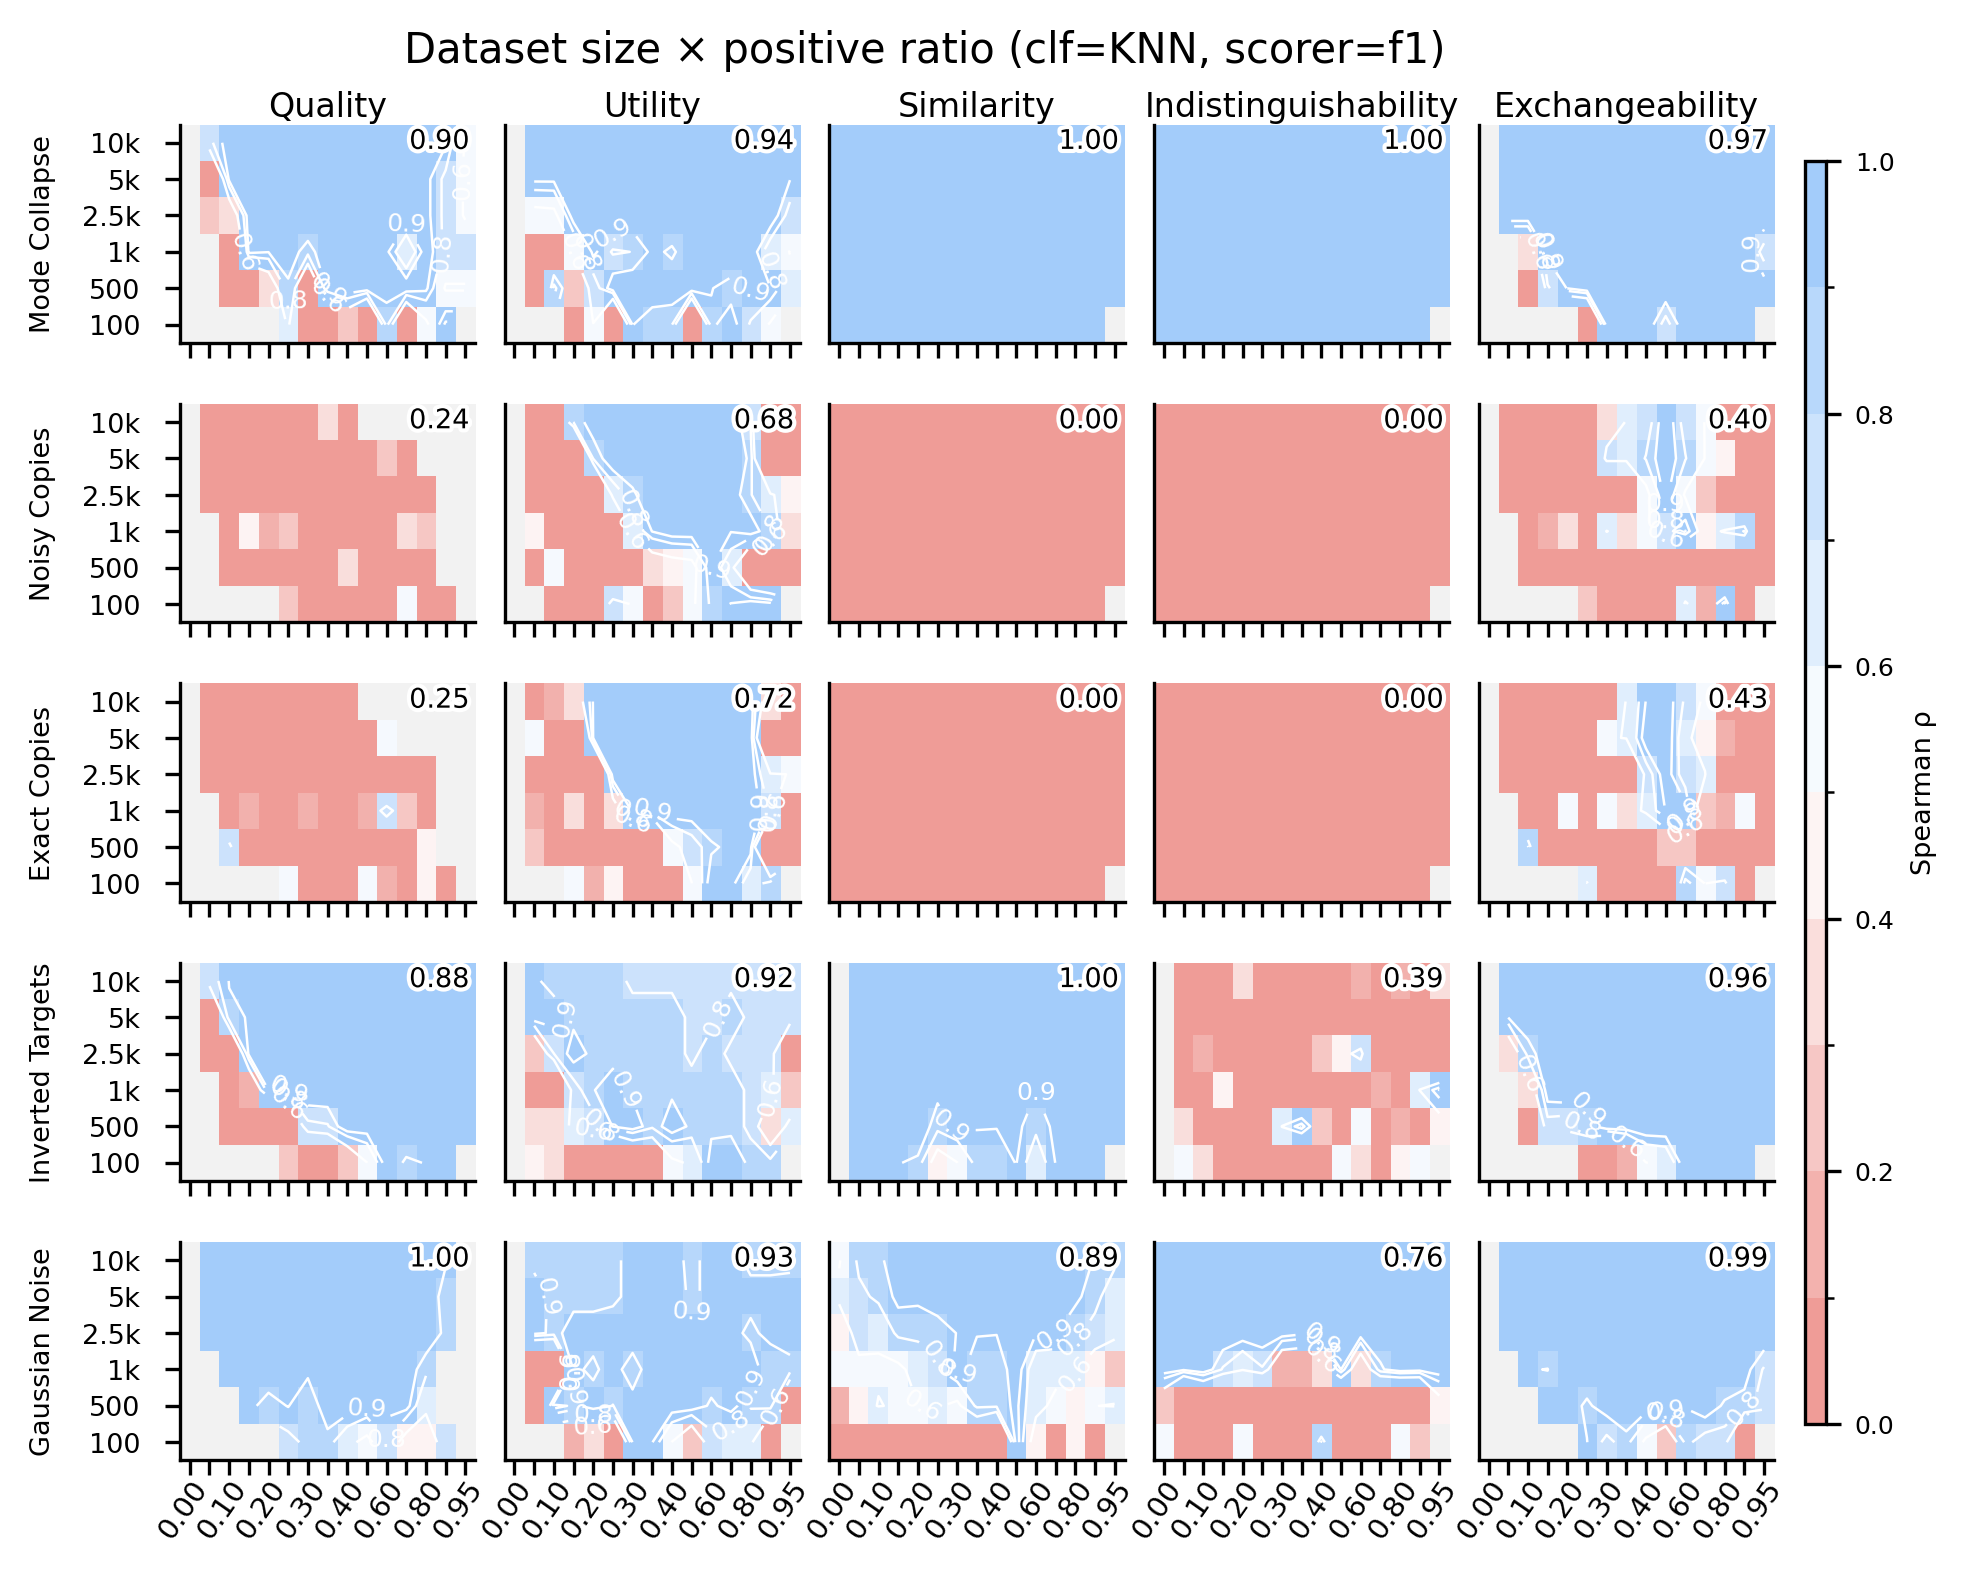
\includegraphics[width=\linewidth]{images/rankgen/synthetic/size_vs_pos.png}% don't set height; keepaspectratio is default
  \caption[Stability maps: size × positive ratio]{Stability maps for \emph{dataset size × positive ratio}
  (clf=KNN, scorer=f1). Color shows Spearman’s $\rho$ (clipped to $[0,1]$); the
  number in each panel is $\widehat{p}_{\mathrm{deg}}=\Pr(\rho>0)$, the fraction of
  grid settings that degrade (smaller is better).}
  \label{fig:size-vs-pos}
\end{figure}

\textbf{Diagnosing Generators via Metric Profiles.}
Figure~\ref{fig:size-vs-pos} illustrates how each quantile-estimated RankGen metric responds to different perturbation types and dataset sizes.
Beyond canonical failure modes, we introduce a novel scenario—\emph{noisy copies}—in which near-duplicates of training samples, lightly corrupted with Gaussian noise, are injected into the generated set.
This case is particularly valuable for testing sensitivity to memorisation.

Each metric offers a distinct diagnostic signal, effectively fingerprinting how a generator fails.
\textbf{Quality} sharply degrades under mode collapse, label flips, and Gaussian noise—revealing poor generalisation.
\textbf{Utility} uniquely detects memorisation in the noisy-copy scenario and remains robust across most perturbations.
\textbf{Indistinguishability} is highly sensitive to global shifts and feature corruption but fails to flag copying, where the discriminator underfits.
\textbf{Similarity} captures structural misalignment from label and topology noise, though it too struggles with near-copies.
\textbf{Exchangeability} synthesizes these perspectives into a single, composite view—capturing both task-relevance and distributional alignment.
However, as a consequence of this blending, its behaviour can become non-monotonic in edge cases.
In the noisy-copy setting, for example, utility steadily declines as duplication increases, while similarity paradoxically improves—since noisy copies still resemble the original data.
When these two effects compete, Exchangeability can appear erratic, exposing a tension between structural proximity and task degradation.

\textbf{Comparison with Baseline Metrics.}
As shown in Appendix \ref{appendix:pr_dc}, we also evaluate Coverage/Density~\citep{kynkaanniemi2019improved},
Precision/Recall for distributions~\citep{sajjadi2018assessing},
FID~\citep{heusel2017gans},
MMD (Linear/RBF)~\citep{gretton2012kernel},
and F1-based variants~\citep{powers2011f1}.
While some of these exhibit strong correlations under specific perturbations (e.g., \textbf{F1\_PR} under mode collapse, or \textbf{MMD} under Gaussian noise), their overall sensitivity is limited.
\subsubsection{\textbf{How often classifiers may fail the PAC Bounds}}
Across all synthetic perturbation experiments, Table~\ref{tab:pac-fail-overall} reports how frequently classifier probes failed to satisfy their PAC bounds at $\delta = 0.05$. Failures are relatively rare for tree-based methods (e.g., Random Forests, Gradient Boosting, AdaBoost), which almost always produced statistically reliable estimates across axes. In contrast, some simple classifiers show much higher failure rates: GaussianNB and Logistic Regression violated bounds nearly half the time on the \emph{Utility} and \emph{Exchangeability} axes, while SVC and $k$-NN occasionally failed on \emph{Quality}. These differences highlight that not all classifiers provide equally stable probes. The overall pattern reinforces the value of PAC-style guarantees: they make explicit when a probe’s conclusions are statistically trustworthy, and when they should be treated with caution.
\normalsize
\begin{table}[H]
  \centering
  \footnotesize
  \setlength{\tabcolsep}{3.5pt}
  \renewcommand{\arraystretch}{1.15}
  \begin{tabularx}{\columnwidth}{l *{5}{r}}
    \toprule
    {\textbf{Classifier}} &
    {\makecell{\textbf{Quality}}} &
    {\makecell{\textbf{Utility}}} &
    {\makecell{\textbf{Indistinguishability}}} &
    {\makecell{\textbf{Similarity}}} &
    {\makecell{\textbf{Exchangeability}}} \\
    \midrule
    AdaBoostClassifier         & 0.000 & 0.167 & 0.067 & 0.000 & 0.167 \\
    DecisionTreeClassifier     & 0.006 & 0.167 & 0.042 & 0.000 & 0.167 \\
    ExtraTreesClassifier       & 0.048 & 0.167 & 0.194 & 0.000 & 0.167 \\
    GaussianNB                 & 0.273 & 0.500 & 0.064 & 0.000 & 0.500 \\
    GradientBoostingClassifier & 0.027 & 0.167 & 0.085 & 0.000 & 0.167 \\
    KNeighborsClassifier       & 0.145 & 0.000 & 0.033 & 0.000 & 0.000 \\
    LogisticRegression         & 0.161 & 0.482 & 0.030 & 0.000 & 0.482 \\
    RandomForestClassifier     & 0.048 & 0.167 & 0.124 & 0.000 & 0.167 \\
    SVC                        & 0.215 & 0.000 & 0.048 & 0.000 & 0.000 \\
    \bottomrule
  \end{tabularx}
  \caption{Overall PAC \emph{fail frequency} (proportion) by classifier, aggregated across all synthetic experiments at $\delta=0.05$ (lower is better).}
  \label{tab:pac-fail-overall}
\end{table}

\subsubsection{\textbf{PCA of RankGen Metrics on Synthetic Perturbations}}
\label{sec:pca-synthetic}
\begin{figure}[H]
  \centering
  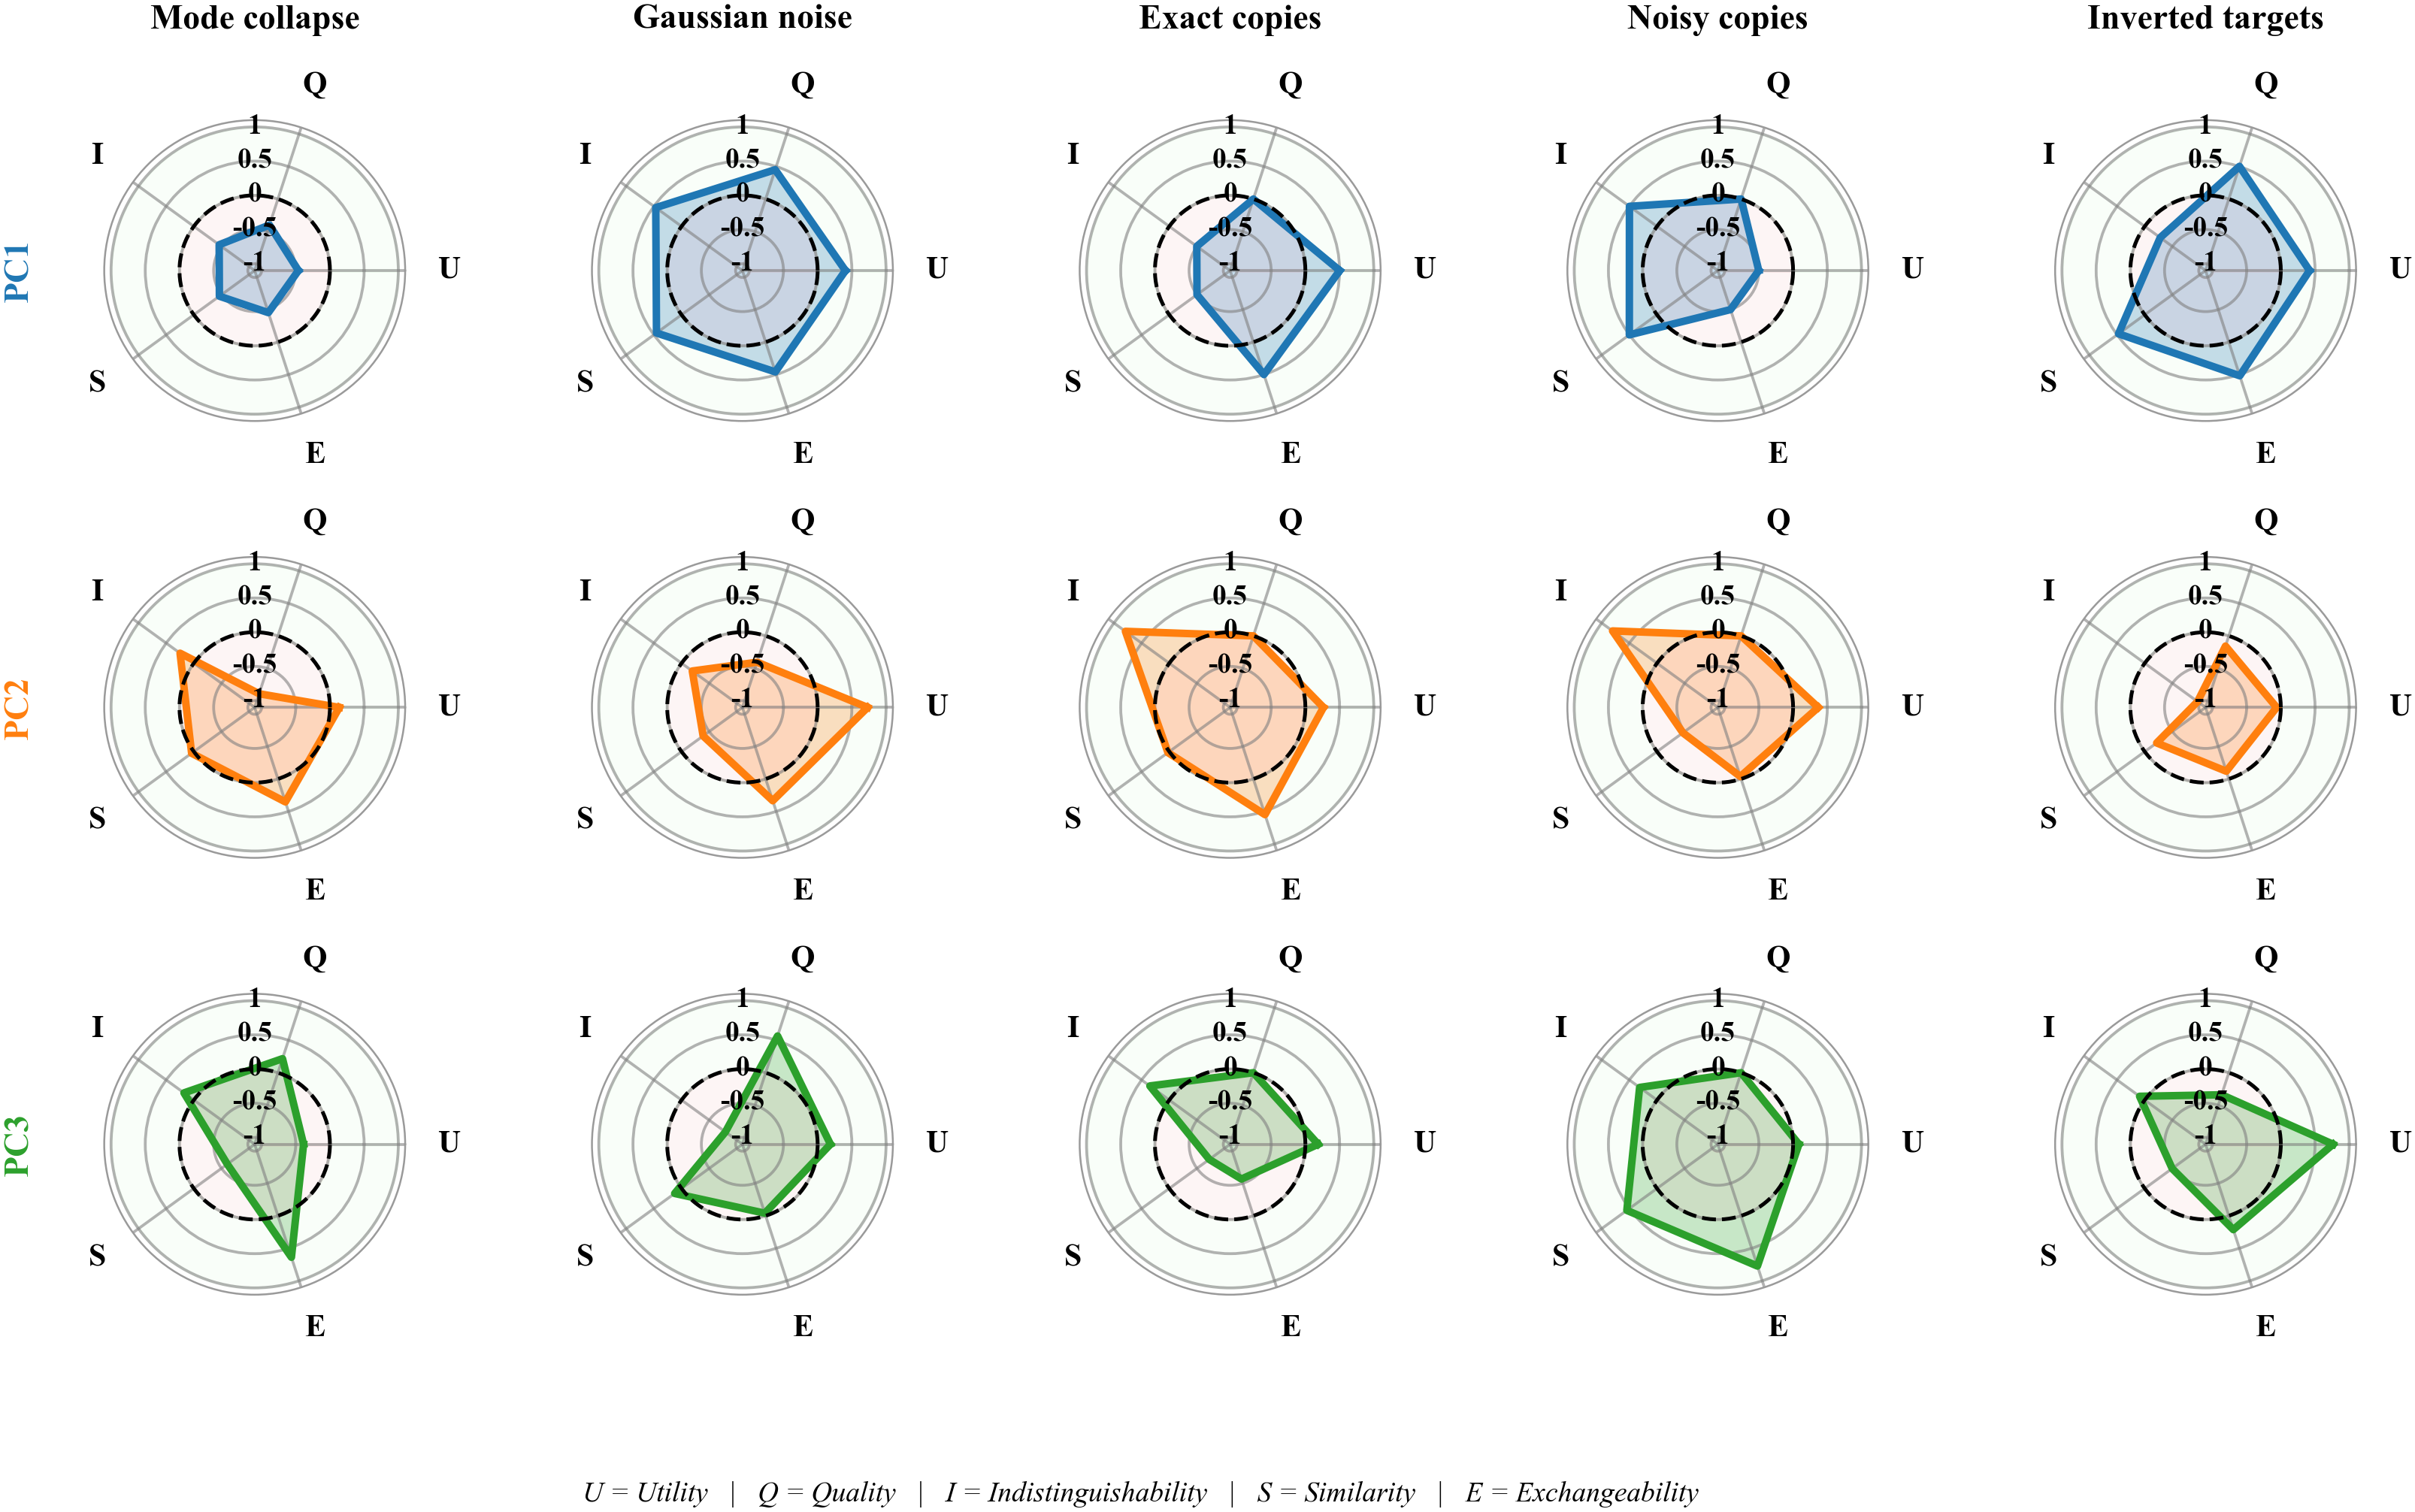
\includegraphics[width=1\linewidth]{images/rankgen/synthetic/radial_plot.png}
  \caption{\textbf{PCA loadings of RankGen metrics under synthetic perturbations.}
  Columns correspond to perturbations (Mode collapse, Gaussian noise, Exact copies, Noisy copies, Inverted targets).
  Rows correspond to principal components (PC1–PC3), color-coded by PC (blue = PC1, orange = PC2, green = PC3).
  Each radar plot shows loadings of $\{U,Q,I,S,\mathcal E_{\min}\}$; the dashed circle marks $0$ (rings at $\pm0.5$ and $\pm1$).
  PC1 captures a global corruption factor, while PC2/PC3 reveal complementary trade-offs (e.g., $Q$ vs.\ $I/E$, or $U$ vs.\ $S$).}
\end{figure}
We apply PCA to standardized metric vectors $(U,Q,I,S,E)$ to study how RankGen’s axes co-vary under canonical perturbations. Standardization (zero mean, unit variance) ensures that principal components reflect \emph{shared structure} rather than differences in raw scale \citep{jolliffe2002pca,abdi2010pca}.

\paragraph{Global factor vs.\ structured trade-offs.}
Across most perturbations, \textbf{PC1} behaves as a global “level” factor: all metrics load in the same direction, capturing overall corruption severity. This pattern is clearest in the Gaussian noise and mode collapse settings, where PC1 explains nearly all variance with uniform contributions from $\{U,Q,I,S,E\}$. By contrast, perturbations involving duplication or label inversion distribute variance across multiple components. In noisy copies and inverted targets, PC1 accounts for a smaller share, leaving PC2/PC3 to isolate distinct residual signals.

\paragraph{Scenario-specific axes.}
The remaining components (PC2, PC3) disentangle complementary trade-offs. For Gaussian noise, PC2 contrasts \textbf{Quality} against \textbf{Indistinguishability} and \textbf{Exchangeability}, while PC3 highlights residual variance in \textbf{Utility}. For mode collapse, PC2/PC3 emphasise losses in \textbf{Similarity} and \textbf{Utility}, consistent with reduced local mixing and predictive value. For exact copies, higher-order axes distinguish between inflated \textbf{Indistinguishability} and depressed \textbf{Utility}/\textbf{Similarity}, reflecting the fact that duplicates look realistic but add little value. In noisy copies, the decomposition shows a more complex balance, with \textbf{Quality} and \textbf{Exchangeability} trading off against \textbf{Similarity}. Finally, in inverted targets, PC2 is dominated by \textbf{Indistinguishability}, while PC3 sets \textbf{Utility} against \textbf{Similarity} and \textbf{Quality}, consistent with models that flip labels being easy to tell apart yet still producing plausible-looking samples.

\paragraph{Interpretation.}
Signs of loadings are arbitrary in PCA \citep{abdi2010pca,lever2017pca}; what matters are their relative magnitudes and oppositions. The fact that PC2/PC3 consistently recover orthogonal axes beyond the global level confirms that RankGen’s metrics are not collinear. Instead, they capture complementary error signatures: once the “common factor” is removed, residual axes reveal whether degradation arises from poor utility, collapsed similarity, or label inversion. This diagnostic separation is precisely what RankGen is designed to provide.



\subsection{Real-World Graph Datasets}
\label{sec:real-world-graphs}
We focus our real-world evaluation on structured domains where human inspection is infeasible—
specifically, molecular graphs. Unlike images, where qualitative assessment is often possible, graphs lack intuitive visual cues, making rigorous, task-relevant evaluation metrics essential. To reflect realistic deployment scenarios where human curation or large-scale pretraining is not viable, we train generative models on relatively small datasets (hundreds to a few thousand instances), simulating low-resource settings common to several scientific domains.

Our datasets are sourced from the \textit{Therapeutics Data Commons}\citep{huang2021tdc}, encompassing a diverse suite of molecular prediction tasks relevant to drug discovery and pharmacology: \textsc{AMES} (mutagenicity prediction), \textsc{BBB} (blood–brain barrier penetration), \textsc{CYP1A2} and \textsc{CYP2C19} (cytochrome P450 enzyme binding), \textsc{hERG} (cardiotoxicity risk via hERG channel inhibition), and \textsc{Lipophilicity} (logP estimation as a proxy for solubility and absorption). Each molecule is originally provided as a SMILES string\citep{weininger1988smiles}, which we convert into graph representations where atoms are nodes and bonds are edges.
\begin{figure}[H]
  \centering
   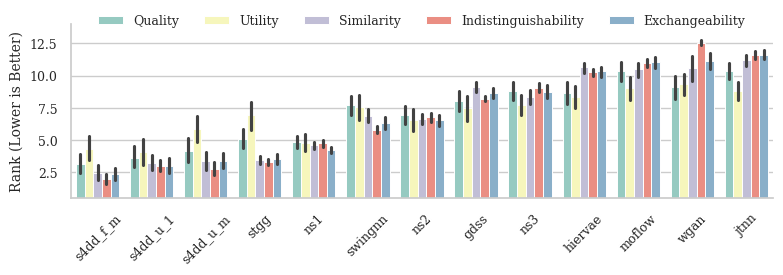
\includegraphics[width=\textwidth]{images/rankgen/real_generators/generators_rank_all_datasets.png}
  \caption{Average generator rank per metric across all datasets and vectorizers. Lower is better.}
  \label{fig:generators-rank}
\end{figure}
For each dataset, we perform class-conditional generation using a diverse set of molecular generative models spanning multiple paradigms. \textbf{STGG}\citep{ahn2021spanning} is an autoregressive model that constructs molecules via spanning trees; \textbf{WGAN-GP with R-GCN}\citep{keras2021wgan} applies adversarial training to graph-structured data; \textbf{JTNN}\citep{jin2018junction} and \textbf{HierVAE}\citep{c} are hierarchical variational autoencoders, the former based on junction trees and the latter on motif assembly; \textbf{MoFlow}\citep{zang2020moflow} is a normalizing flow model allowing exact likelihood estimation; \textbf{GDSS}\citep{jo2022score} is a score-based diffusion model built on stochastic differential equations; and \textbf{SWINGNN}\citep{yan2023swingnn} is a graph diffusion model enhanced with shifted window attention. We also introduce the \textbf{Neighborhood Swap Generator (NS)}, a non-parametric, training-free method that perturbs input graphs through iterative local rewiring of neighbourhood subgraphs, producing diverse synthetic variants across one to three rounds of compounding perturbations (NS-1, NS-2, NS-3). These models collectively span autoencoding, flow-based, adversarial, diffusion-based, and perturbation-based generative paradigms (see Appendix~\ref{appendix:molecular_datasets} and Appendix~\ref{appendix:hyperparameters_for_molecular} for details).

\textbf{Feature Representation.}
To enable consistent comparison, we convert molecular graphs into fixed-length vectors using three types of encoders: (1) classical fingerprints (e.g., \textbf{Morgan}, \textbf{Torsion}, \textbf{Atom Pair}, \textbf{RDKit}\citep{rdkit2011}); (2) neural graph embeddings from models such as \textbf{GIN}\citep{xu2019powerful}, \textbf{GraphCL}\citep{you2020graph}, and \textbf{InfoGraph}\citep{sun2019infograph}; and (3) discrete graph kernels, notably \textbf{NSPDK}~\citep{costa2010fast}. This diversity supports robust evaluation across both learned and handcrafted feature spaces. While overall trends are consistent, we observe that the choice of vectorizer can influence generator rankings within each PAC-valid group, highlighting the importance of feature representation in shaping performance signals.
\paragraph{Model Comparison Across Real Generators.}
Figure~\ref{fig:generators-rank} displays the average quantile-based ranking of each generator, aggregated across datasets and feature encodings.\footnote{Table~\ref{tab:bounds_check} reflects a single experimental run (see Fig.\ref{fig:rank_herg_karim}), while Fig.\ref{fig:generators-rank} averages over multiple trials—accounting for observed differences.} \textbf{S4DD} variants and \textbf{STGG} consistently achieve top rankings across all metrics, indicating strong generalisation and distributional alignment. In contrast, models such as \textbf{WGAN} and \textbf{MoFlow} rank poorly—particularly in \textbf{Exchangeability}—suggesting limited task utility and diversity.
Interestingly, the pretrained version of S4DD—trained on over a million molecules—does not yield substantial gains over its dataset-specific counterparts trained on only a few thousand examples. This suggests that broad pretraining does not necessarily translate into better generative performance under task-specific constraints.
These findings reinforce RankGen’s central insight: matching superficial distributional statistics is not enough. While some models may inflate conventional metrics through memorisation, \textbf{Exchangeability} penalizes such behaviour by jointly evaluating utility and alignment—providing a more trustworthy, single-score summary for model selection.


\subsection{Image Benchmarks: MNIST, Fashion--MNIST, and CIFAR--10}
\label{sec:image-benchmarks}
\begin{figure}[H]
  \centering
  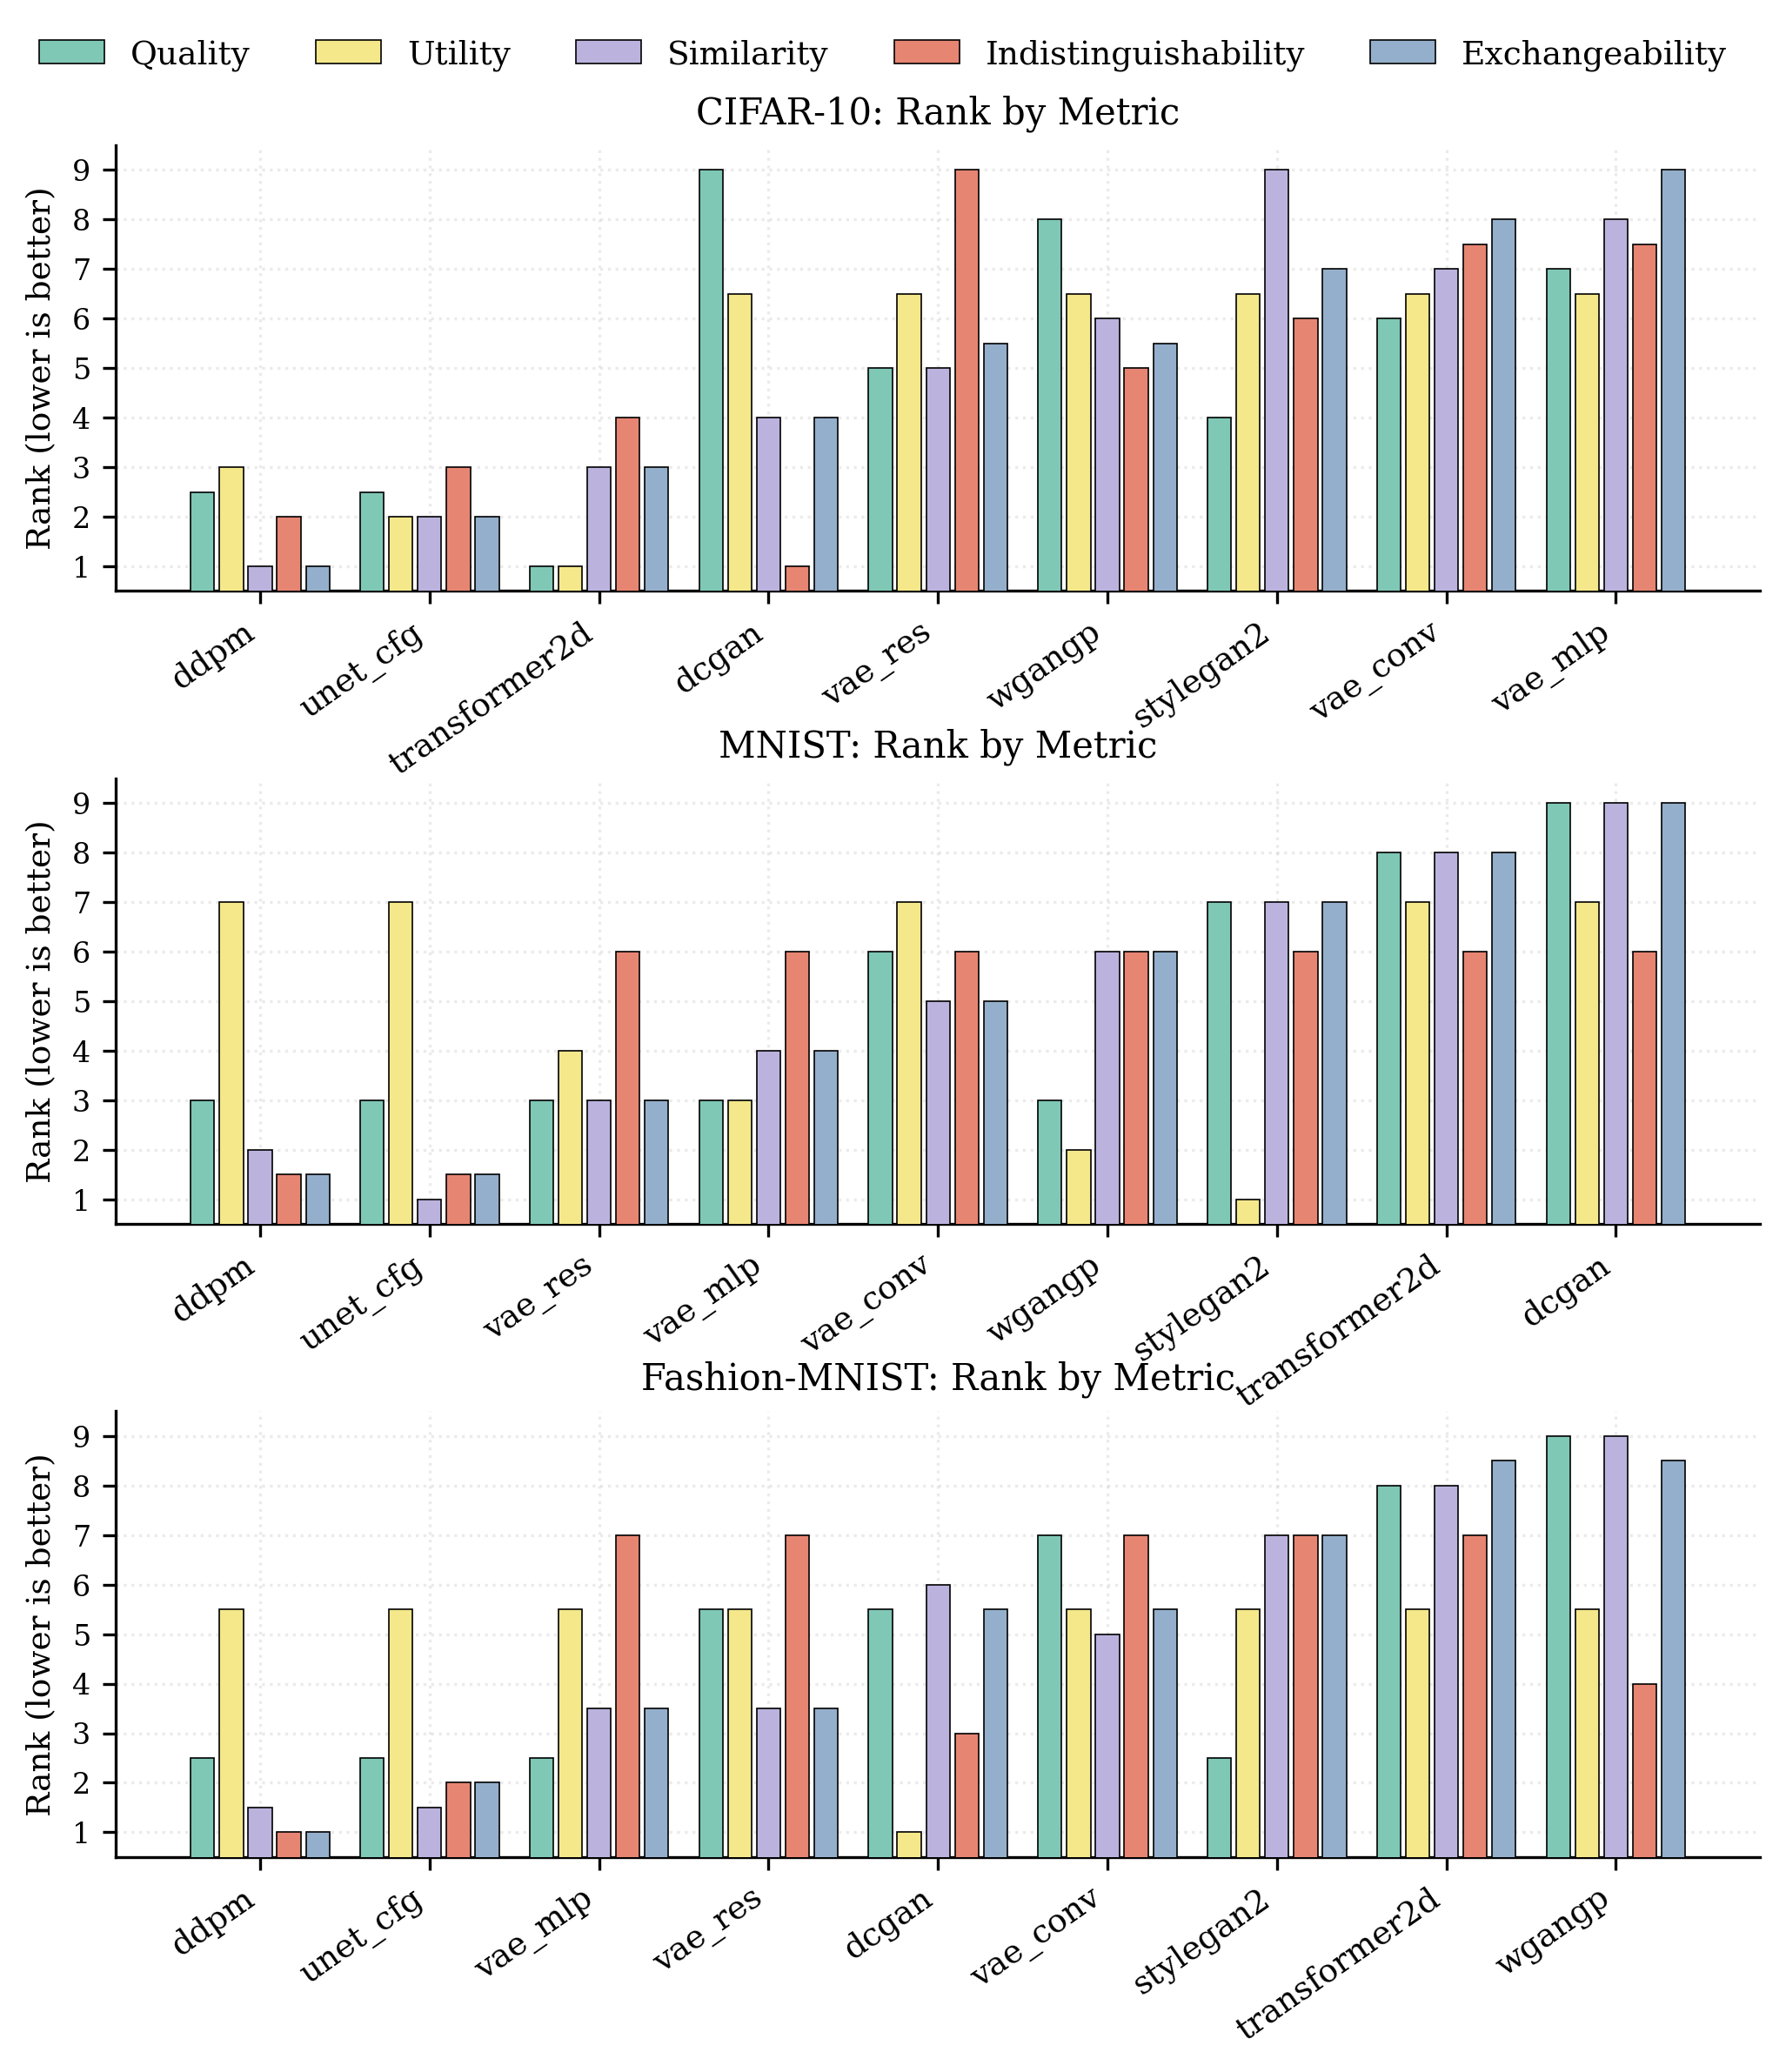
\includegraphics[width=0.80\linewidth,height=1.5\textheight,keepaspectratio]{images/rankgen/real_generators/rank_images.png}
  \caption{RankGen ranks on \textbf{CIFAR--10}, \textbf{MNIST}, and \textbf{Fashion--MNIST}.
  Lower is better. StyleGAN2-lite exhibits high Quality but low Utility and Similarity, echoing our synthetic mode-collapse setting. This suggests strong precision but poor coverage—models of this type risk overfitting narrow regions of the data. VAEs remain competitive on digits.}
  \label{fig:cifar10-ranks}
\end{figure}
We use three canonical benchmarks: \textbf{MNIST}~\citep{lecun1998gradient},
\textbf{Fashion--MNIST}~\citep{xiao2017fashion}, and \textbf{CIFAR--10}~\citep{krizhevsky2009learning},
with consistent preprocessing and stratified splits (Appendix~\ref{app:image-experiments}).
Test images are never used for training or selection. We evaluate class-conditional generators spanning multiple paradigms.
\textbf{VAEs:} MLP-VAE, Conv-VAE, and ResNet-VAE~\citep{kingma2014auto,rezende2014stochastic}.
\textbf{GANs:} DCGAN~\citep{radford2016unsupervised}, WGAN--GP with projection discriminator~\citep{gulrajani2017improved,miyato2018cgans}, and a $32{\times}32$ \textbf{StyleGAN2-lite}~\citep{karras2020analyzing}.
\textbf{Diffusion:} cDDPM with UNet backbone~\citep{ho2020denoising,ronneberger2015u,ho2022classifier} and a Transformer2D backbone (DiT style)~\citep{peebles2023di}, using HuggingFace Diffusers samplers~\citep{von-platen-etal-2022-diffusers} (see architectural and training details  in Appendix~\ref{app:image-models}).
\paragraph{RankGen summary and diagnostics.}
Figure~\ref{fig:cifar10-ranks} summarizes generator \emph{ranks} under RankGen
(Quality $Q$, Utility $U$, Indistinguishability $I$, Similarity $S$, and Exchangeability $E$)
across datasets. Several consistent patterns emerge.

\textit{First}, diffusion models are the only family that consistently balances all four base metrics,
achieving strong overall Exchangeability. They dominate $Q$ and $S$ across datasets, reflecting high visual fidelity
and broad distributional coverage, which is also evident in the sample panels.

\textit{Second}, GAN-based models exhibit clear trade-offs.
\texttt{stylegan2} attains high $Q$ but shows weak $U$ and $S$, consistent with a high-precision/low-recall regime
characteristic of mode collapse: samples are sharp but lack diversity and task utility.
Conversely, \texttt{dcgan} achieves strong $I$ while remaining near chance in $U$, indicating that although samples may appear realistic,
they provide limited augmentation value. These patterns highlight how single-number heuristics (e.g., IS)
can obscure important failure modes.

\textit{Third}, VAEs underperform on CIFAR--10 due to reduced $Q$ and $U$, reflecting blur and limited diversity,
but remain competitive on MNIST and Fashion--MNIST, where lower complexity and grayscale structure better match their inductive bias.

Overall, RankGen reveals distinct architectural ``fingerprints'', diagnosing failure modes that are otherwise flattened by aggregate scores.
The underlying metric values are reported in Appendix~\ref{app:image-results}, with illustrative samples shown in
Figures~\ref{fig:cifar10_generated_panel}, \ref{fig:fashionmnist_generated_panel}, and \ref{fig:mnist_generated_panel}
(Appendix~\ref{appendix:example}).
We further compare RankGen to standard metrics such as FID, KID, PRD, and VENDI
(Tables~\ref{tab:vals-ranks-cifar10}--\ref{tab:ke-mnist-ranked}), observing broad agreement in well-behaved regimes
(e.g., diffusion models ranking highest), alongside informative divergences in settings where classical metrics are known to be less reliable.


\subsection{RankGen and Conventional Image Metrics}
\label{sec:rankgen-vs-conventional}

To contextualize the RankGen scores, we compare them against standard image
evaluation metrics and kernel--entropy diversity proxies. Figure~\ref{fig:mnist-ranks}
reports Spearman correlations between per-generator ranks under RankGen and
under conventional image metrics, while the full numeric results are deferred to
Appendix~\ref{app:image-results}.

\paragraph{Conventional image metrics.}
We report FID~\citep{heusel2017gans}, KID~\citep{binkowski2018demystifying},
precision/recall for distributions and their harmonic mean
(\textbf{F1\_pr})~\citep{sajjadi2018assessing,kynkaanniemi2019improved}, and
Inception Score (IS)~\citep{salimans2016improved}, using
$n_{\text{ref}}=n_{\text{gen}}$ as indicated. Across datasets, diffusion models
(\texttt{ddpm}, \texttt{unet\_cfg}) achieve the best or near-best FID/KID and
the strongest F1\_pr, while \texttt{stylegan2} exhibits high precision but very
low recall, consistent with mode dropping. VAEs underperform on CIFAR--10 but
remain more competitive on MNIST and Fashion--MNIST. Full results with
per-metric ranks are reported in
Tables~\ref{tab:cifar10-ranked}--\ref{tab:mnist-ranked}.

\paragraph{Kernel--entropy diversity proxies.}
To complement embedding-based distances, we also compute kernel--entropy
proxies of sample diversity: VENDI/RKE surrogates estimated via FKEA
(RKE\_gen, FKEA--VENDI\_gen, FKEA--RKE2\_gen) and the reference-relative
variant RRKE (lower is better)~\citep{friedman2023vendi,pasarkar2024cousins,jalali2024fkea,luo2024converge}.
Per-dataset results and kernel widths $\sigma$ are given in
Tables~\ref{tab:ke-cifar10-ranked}--\ref{tab:ke-mnist-ranked}. Diffusion models
again rank highest, showing higher entropy and lower redundancy, while VAEs
show reduced entropy and GANs occupy an intermediate regime. As discussed in
Sec.~\ref{sec:related:evaluation}, these spectral scores are useful for
detecting mode collapse, but they remain label- and task-agnostic and operate
primarily on the generated set, so they cannot by themselves diagnose copying
or augmentation value.

\paragraph{Relationship to RankGen.}
Figure~\ref{fig:mnist-ranks} shows that RankGen is broadly consistent with
conventional metrics where expected, but provides additional diagnostic
resolution. In particular, RankGen $Q$ and $S$ align closely with precision and
recall, while exchangeability $\mathcal{E}_{\min}$ aligns most strongly with
$F1_{\text{pr}}$, indicating that the composite captures both fidelity and
coverage. By contrast, IS exhibits weaker and less consistent agreement. This
agreement is strongest on MNIST, but remains qualitatively stable across all
three datasets.

The key advantage of RankGen appears precisely in the cases where conventional
metrics disagree or become ambiguous. Diffusion models rank near the top under
both metric families, but models such as StyleGAN2 and WGAN--GP reveal the
added value of RankGen’s task-aware probes. StyleGAN2 achieves competitive
FID/KID and high precision, yet RankGen assigns it low Utility and low
Similarity, exposing its concentrated, mode-dropping behaviour. WGAN--GP
obtains middling conventional scores, but RankGen identifies near-zero Utility,
indicating that its samples add little task-relevant information despite
appearing plausible in feature space. Likewise, VAEs may remain moderately
ranked by FID/KID on simpler datasets, but RankGen exposes their weaker task
fidelity and augmentation value, especially on CIFAR--10.

Overall, conventional metrics capture global similarity and diversity, whereas
RankGen additionally measures task fidelity, augmentation value, local mixing,
and copying sensitivity. The two families are therefore best viewed as
complementary: conventional metrics provide broad distributional summaries,
while RankGen explains \emph{why} generators with similar global scores can
behave very differently in downstream use.

\begin{figure}[H]
  \centering
  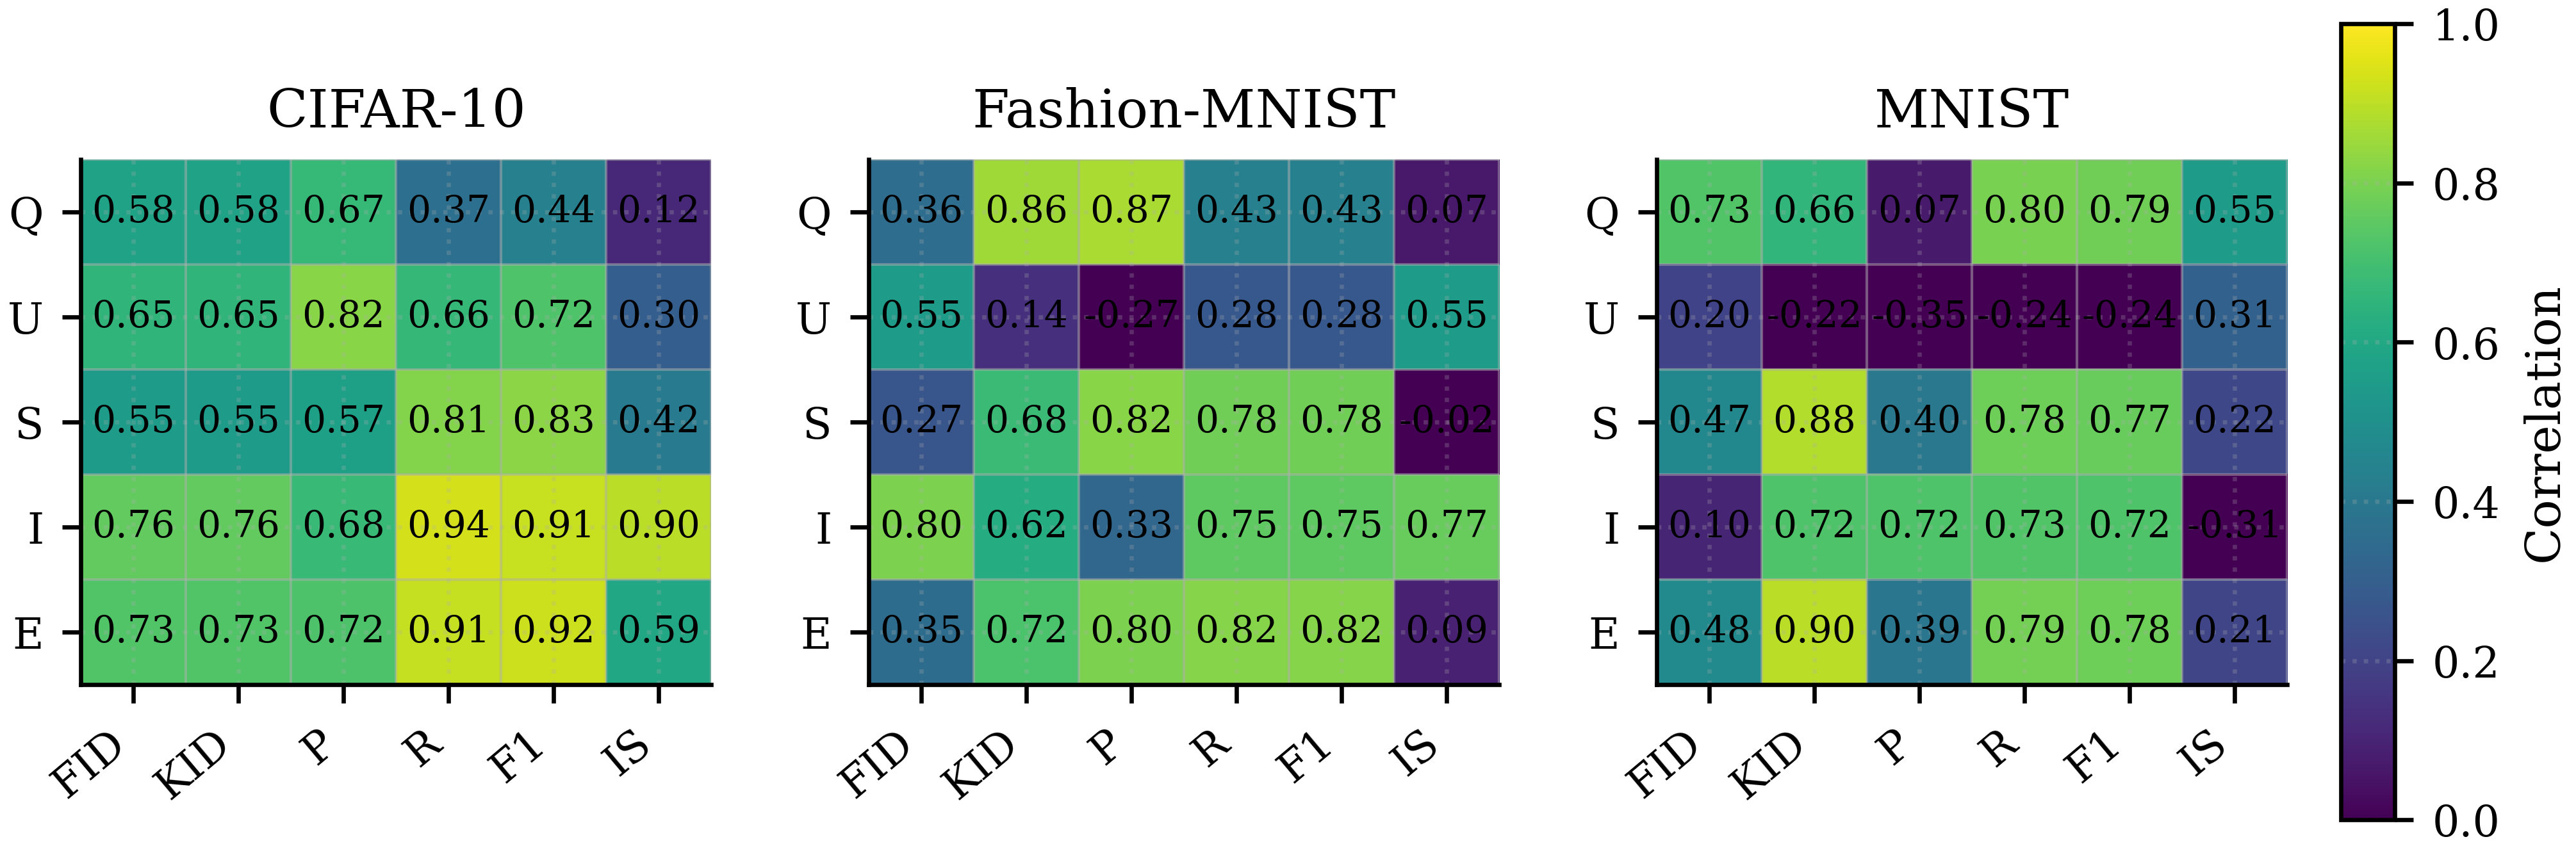
\includegraphics[width=\linewidth,height=0.82\textheight,keepaspectratio]{images/rankgen/real_generators/rank_corr_3panel.png}
  \caption{\textbf{RankGen vs.\ conventional metrics (by dataset).}
  Cells show Spearman correlations between RankGen metrics
  ($Q,U,S,I,\mathcal{E}_{\min}$) and conventional metrics
  (FID, KID, P, R, $F_{1,\mathrm{pr}}$, IS) on \textbf{CIFAR--10},
  \textbf{Fashion--MNIST}, and \textbf{MNIST}. RankGen $Q$ and $S$ track
  precision and recall, while exchangeability aligns most closely with
  $F_1$. IS shows the weakest alignment.}
  \label{fig:mnist-ranks}
\end{figure}
\subsection{Open-Domain Text Generation}
\label{subsec:text}

To assess whether \textsc{RankGen} generalises beyond graph and image generators, we evaluate it on open-domain text generation using the \textsc{AG-News} corpus~\citep{zhang2015character}, which contains news headlines labelled with four topics (\emph{World}, \emph{Sports}, \emph{Business}, \emph{Sci/Tech}). We treat human-written headlines as real data and consider three GPT-2 variants~\citep{radford2019language} as conditional generators: \texttt{distilgpt2}, \texttt{gpt2}, and \texttt{gpt2-medium}. For each class, models are prompted with a topic-specific prefix and used to sample synthetic headlines.

All real and generated headlines are embedded using a frozen MiniLM sentence encoder~\citep{wang2020minilm}, and \textsc{RankGen} is applied with a logistic regression classifier as the downstream estimator, following the same protocol as in previous sections.

\textsc{RankGen} clearly differentiates the three generators and recovers the expected capacity ordering:

\begin{table}[t]
\centering
\small
\begin{tabular}{lcccc}
\toprule
\textbf{Model} & \textbf{F1} & \textbf{Quality} & \textbf{Indist.} & \textbf{Similarity} \\
\midrule
\texttt{distilgpt2} & 0.38 & 0.48 & 0.04 & 0.17 \\
\texttt{gpt2} & 0.45 & 0.57 & 0.08 & 0.24 \\
\texttt{gpt2-medium} & 0.45 & 0.57 & 0.09 & 0.26 \\
\bottomrule
\end{tabular}
\caption{Open-domain text generation results on \textsc{AG-News}.}
\label{tab:text-results}
\end{table}

\[
\texttt{distilgpt2} \;<\; \texttt{gpt2} \;<\; \texttt{gpt2-medium}.
\]

Across metrics, larger models achieve higher Quality, Similarity, and Indistinguishability (Table~\ref{tab:text-results}), while real-versus-generated classification accuracy remains below perfect ($\approx 0.96$, $0.92$, $0.91$), ruling out trivial separability and indicating partial overlap between real and synthetic samples in representation space.

These results show that \textsc{RankGen} generalises to high-dimensional text generation without any text-specific modifications to the method.
\section{Conclusion}
\label{sec:conclusion-rankgen}
This chapter introduced \textsc{RankGen}, a statistically grounded framework for
evaluating generative models through complementary classifier-based probes rather
than through a single heuristic score. The central premise is that generative
model evaluation should be treated as a learning problem: different predictive
tasks reveal different failure modes, and empirical scores should be interpreted
together with explicit uncertainty control.

To operationalize this idea, RankGen combines four metrics---\emph{Quality},
\emph{Utility}, \emph{Indistinguishability}, and \emph{Similarity}---with
PAC-style reliability bounds, robust quantile-based summaries, and a two-stage
ranking procedure. This yields an evaluation protocol that first filters out
statistically unreliable generators and then ranks the remaining candidates in
an uncertainty-aware manner. The resulting composite,
\emph{Exchangeability}, provides a conservative summary of whether a generator is
both predictively useful and distributionally aligned.

The empirical results show that this framework is not only descriptive but
diagnostic. On controlled synthetic perturbations, RankGen responds
systematically to memorisation, mode collapse, label corruption, and geometric
misalignment, with different metrics isolating different pathologies. On
molecular graph datasets, it separates generators that merely resemble the data
distribution from those that provide meaningful task-relevant signal. On image
benchmarks, it remains broadly consistent with conventional measures such as
FID, KID, and precision--recall, while adding information those scores do not
capture---most notably augmentation value, local mixing, and copying
sensitivity.

Taken together, these results support the broader claim of the chapter:
generative model evaluation should not be understood as the computation of a
single scalar similarity measure, but as a statistically controlled,
multi-dimensional inference problem. RankGen provides one concrete realization
of this view, offering a practical framework for reliable model comparison in
settings where downstream utility, robustness, and safety matter.
